\documentclass[12pt,a4paper]{article}
\usepackage[a4paper, margin=0.8in, headheight=14pt]{geometry}
\usepackage{fontspec}
\usepackage{unicode-math}
\setmainfont{TeX Gyre Pagella}
\setmonofont[Scale=0.88]{TeX Gyre Cursor}
\setmathfont{Latin Modern Math}
\usepackage{xcolor}
\usepackage{colortbl}
\usepackage{titlesec}
\usepackage{enumitem}
\usepackage{tabularx}
\usepackage{booktabs}
\usepackage{array}
\usepackage{amsmath}
\usepackage{tikz}
\usetikzlibrary{shapes.geometric, arrows.meta, positioning, calc, fit, decorations.pathreplacing, decorations.pathmorphing}
\usepackage{tcolorbox}
\tcbuselibrary{skins, breakable}
\usepackage{hyperref}
\usepackage{fancyhdr}
\usepackage{graphicx}
\usepackage{microtype}
\hyphenpenalty=10000
\exhyphenpenalty=10000
\sloppy
\usepackage{caption}
\usepackage{setspace}
\usepackage{multirow}
\usepackage{tocloft}
\newcommand{\Q}[1]{\textbf{#1}\par\noindent\ignorespaces}
\definecolor{myred}{RGB}{196,30,58}
\definecolor{mydark}{RGB}{30,30,50}
\definecolor{mygreen}{RGB}{14,120,80}
\definecolor{myteal}{RGB}{0,130,140}
\definecolor{myamber}{RGB}{180,100,0}
\definecolor{mypurple}{RGB}{100,30,160}
\definecolor{mygray}{RGB}{246,247,249}
\definecolor{mgframe}{RGB}{180,185,200}
\definecolor{watermark}{RGB}{145,150,170}
\definecolor{hdrred}{RGB}{250,232,235}
\definecolor{hdrgreen}{RGB}{220,244,233}
\definecolor{hdrteal}{RGB}{220,242,244}
\definecolor{hdramber}{RGB}{253,242,215}
\definecolor{hdrpurple}{RGB}{238,228,255}
\definecolor{hdrgray}{RGB}{238,240,245}
\definecolor{rowalt}{RGB}{250,251,253}

\titleformat{\section}{\large\bfseries\color{myred}}{\thesection.}{0.5em}{}[\vspace{1pt}{\color{myred}\rule{\linewidth}{0.8pt}}]
\titleformat{\subsection}{\normalsize\bfseries\color{myteal}}{\thesubsection}{0.5em}{}
\titlespacing*{\section}{0pt}{18pt}{7pt}
\titlespacing*{\subsection}{0pt}{11pt}{4pt}
\setlength{\parindent}{0pt}
\setlength{\parskip}{4pt}
\renewcommand{\cfttoctitlefont}{\large\bfseries\color{myred}}
\renewcommand{\cftaftertoctitle}{\par\noindent{\color{myred}\rule{\linewidth}{0.8pt}}}
\setlength{\cftbeforetoctitleskip}{0pt}
\setlength{\cftaftertoctitleskip}{6pt}
\renewcommand{\cftsecfont}{\normalsize\bfseries\color{mydark}}
\renewcommand{\cftsecpagefont}{\normalsize\bfseries\color{mydark}}
\renewcommand{\cftsecleader}{\cftdotfill{\cftdotsep}}
\setlength{\cftbeforesecskip}{7pt}
\renewcommand{\cftsubsecfont}{\small\color{mydark}}
\renewcommand{\cftsubsecpagefont}{\small\color{mydark}}
\setlength{\cftbeforesubsecskip}{3pt}
\setlength{\cftsubsecindent}{1.4em}
\renewcommand{\cftpartfont}{\normalsize\bfseries\color{myteal}}
\renewcommand{\cftpartpagefont}{\normalsize\bfseries\color{myteal}}
\setlength{\cftbeforepartskip}{14pt}
\renewcommand{\arraystretch}{1.45}
\setlength{\tabcolsep}{6pt}
\arrayrulecolor{mydark}
\newcolumntype{B}[1]{>{\small\bfseries\raggedright\arraybackslash}m{#1}}
\newcolumntype{C}[1]{>{\centering\arraybackslash}m{#1}}
\newcolumntype{Y}{>{\small\raggedright\arraybackslash}X}
\renewcommand{\tabularxcolumn}[1]{m{#1}}
\newcommand{\currmodule}{Module 1}
\pagestyle{fancy}
\fancyhf{}
\fancyhead[L]{\small\color{myred}\textbf{PE-EC701B}\;\color{mydark}--- Satellite Communication}
\fancyhead[R]{\small\color{myteal}\textbf{\currmodule\ Notes}}
\fancyfoot[C]{\small\color{mydark}\thepage}
\fancyfoot[R]{\small\color{watermark}\textit{\copyright\ Biraj}}
\renewcommand{\headrulewidth}{0.5pt}
\renewcommand{\footrulewidth}{0.3pt}

\hypersetup{colorlinks=true, linkcolor=myteal, urlcolor=myteal,
  pdfauthor={Biraj Sarkar},
  pdftitle={PE-EC701B --- Combined Notes}}

\tcbset{
  tikzbox/.style={
    colback=mygray, colframe=mgframe, boxrule=0.6pt, arc=4pt,
    left=8pt, right=8pt, top=6pt, bottom=6pt,
    colbacktitle=mgframe, coltitle=mydark,
    fonttitle=\small\bfseries
  },
  defbox/.style={
    colback=hdrgreen, colframe=mygreen, boxrule=0.8pt, arc=4pt,
    left=9pt, right=9pt, top=6pt, bottom=6pt,
    colbacktitle=mygreen, coltitle=white,
    fonttitle=\small\bfseries
  },
  formulabox/.style={
    colback=hdrteal, colframe=myteal, boxrule=0.8pt, arc=4pt,
    left=9pt, right=9pt, top=7pt, bottom=7pt,
    colbacktitle=myteal, coltitle=white,
    fonttitle=\small\bfseries
  },
  examplebox/.style={
    colback=hdramber, colframe=myamber, boxrule=0.8pt, arc=4pt,
    left=9pt, right=9pt, top=6pt, bottom=6pt,
    colbacktitle=myamber, coltitle=white,
    fonttitle=\small\bfseries
  },
  masonbox/.style={
    colback=hdrpurple, colframe=mypurple, boxrule=0.8pt, arc=4pt,
    left=9pt, right=9pt, top=6pt, bottom=6pt,
    colbacktitle=mypurple, coltitle=white,
    fonttitle=\small\bfseries
  },
  exambox/.style={
    colback=hdrpurple, colframe=mypurple, boxrule=1pt, arc=5pt,
    left=10pt, right=10pt, top=8pt, bottom=8pt,
    colbacktitle=mypurple, coltitle=white,
    fonttitle=\bfseries,
    breakable, title after break={\textbf{Frequently Asked / Viva Questions (contd.)}}}
}
\tcbset{breakable}
\tcbset{after={\color{black}}}

\tikzset{
  block/.style={rectangle, draw=myteal, fill=hdrteal,
    text width=2.4cm, align=center, minimum height=0.95cm,
    font=\small, rounded corners=3pt, line width=0.7pt},
  redblock/.style={rectangle, draw=myred, fill=hdrred,
    text width=2.4cm, align=center, minimum height=0.95cm,
    font=\small, rounded corners=3pt, line width=0.7pt},
  netnode/.style={rectangle, draw=myteal, fill=hdrteal,
    text width=1.5cm, align=center, minimum height=0.8cm,
    font=\small, rounded corners=3pt, line width=0.7pt},
  sumjunc/.style={circle, draw=myamber, fill=hdramber,
    minimum size=0.62cm, font=\small, line width=0.8pt},
  snode/.style={circle, draw=mypurple, fill=hdrpurple,
    minimum size=0.55cm, font=\footnotesize, line width=0.7pt},
  arrow/.style={-Stealth, thick, color=mydark},
  redarrow/.style={-Stealth, thick, color=myred},
  line/.style={thick, color=mydark}
}

\newcommand{\modulestart}[2]{%
  \clearpage
  \renewcommand{\currmodule}{Module #1}%
  \renewcommand{\theHsection}{mod#1.\arabic{section}}%
  \renewcommand{\theHsubsection}{\theHsection.\arabic{subsection}}%
  \renewcommand{\theHsubsubsection}{\theHsubsection.\arabic{subsubsection}}%
  \phantomsection
  \addcontentsline{toc}{part}{Module #1: #2}%
  \setcounter{section}{0}%
  \begin{center}
    \vspace*{1.0cm}
    {\Huge\bfseries\color{myred} Module #1}\\[10pt]
    {\Large\bfseries\color{mydark} #2}\\[10pt]
    {\color{myred}\rule{0.55\linewidth}{1.2pt}}
  \end{center}
  \vspace{14pt}
}
\begin{document}

\thispagestyle{empty}
\vspace*{1.0cm}
\begin{center}
  {\Huge\bfseries\color{myred} PE-EC701B}\\[10pt]
  {\LARGE\bfseries\color{mydark} Satellite Communication}\\[20pt]
  {\color{myred}\rule{0.7\linewidth}{1.5pt}}\\[18pt]
  {\Large\color{myteal}\textbf{Combined Module Notes}}\\[8pt]
  {\large\color{mydark} Modules 1 -- 6}\\[40pt]
  {\normalsize\color{mydark} Semester VII \quad$\bullet$\quad 3L:0T:0P \quad$\bullet$\quad 3 Credits}\\[12pt]
  {\normalsize\color{mydark} CGEC \;$|$\; B.Tech ECE (2023--27)}\\[6pt]
  {\normalsize\color{mydark}\textit{Biraj Sarkar}}
\end{center}
\vspace{1.0cm}
\begin{center}
  \begin{tcolorbox}[colback=mygray, colframe=mgframe, boxrule=0.5pt, arc=3pt, width=0.85\linewidth]
    \centering\small\color{mydark}
    \textbf{Disclaimer / Study Guide Notice:}\\
    These are condensed \textbf{Short Notes} focusing on core theory, key formulas, block/circuit diagrams, and standard viva Q\&As for university exam revision. Exhaustive numerical practice problems and derivation edge cases are not covered. This serves as a quick-revision reference guide for students.
  \end{tcolorbox}
\end{center}
\vfill
\begin{center}{\small\color{watermark}\textit{Exam-Ready Notes}}\end{center}
\clearpage

\hypersetup{linkcolor=mydark}
\tableofcontents
\hypersetup{linkcolor=myteal}
\clearpage

% -- Module 1 -----------------------------------------------------------------
\modulestart{1}{Principles of Satellite Communication}

\section{Principles of Satellite Communication}
% ===============================================================================

Satellite communication is the transmission of information between terrestrial stations using an artificial satellite positioned in Earth's orbit as an active relay. The satellite acts as an orbit-based radio repeater (transponder) that receives signals from one ground station, processes them, and retransmits them to other ground stations.

\begin{tcolorbox}[defbox]
\textbf{Satellite Communication:} A system where an orbiting spacecraft serves as an active wireless relay station. It receives line-of-sight uplink radio signals at frequency $f_u$ from an Earth station, amplifies and translates them to downlink frequency $f_d$, and broadcasts them back to Earth stations.
\end{tcolorbox}

\subsection{Basic Principles of Operation}
The operational principles of a satellite communications system are governed by the following sequence:
\begin{enumerate}[label=\textbf{\arabic*.}, leftmargin=*, itemsep=3pt]
  \item \textbf{Uplink Transmission:} Terrestrial transmitter sends a modulated high-frequency carrier wave (typically in GHz) toward the satellite using a high-gain directional dish antenna.
  \item \textbf{Frequency Translation:} The satellite transponder down-converts the incoming signal to a lower frequency. This translation is vital because it prevents the high-power downlink signal from feeding back and jamming the sensitive uplink receiver.
  \item \textbf{Downlink Transmission:} The converted signal is amplified (via traveling-wave tubes or solid-state power amplifiers) and beamed back to Earth using onboard directive antennas.
\end{enumerate}

\subsection{System Architecture}
The block diagram below details the basic architecture of a satellite communication system:

\begin{tcolorbox}[tikzbox, title={Satellite Communication System Architecture}]
\centering
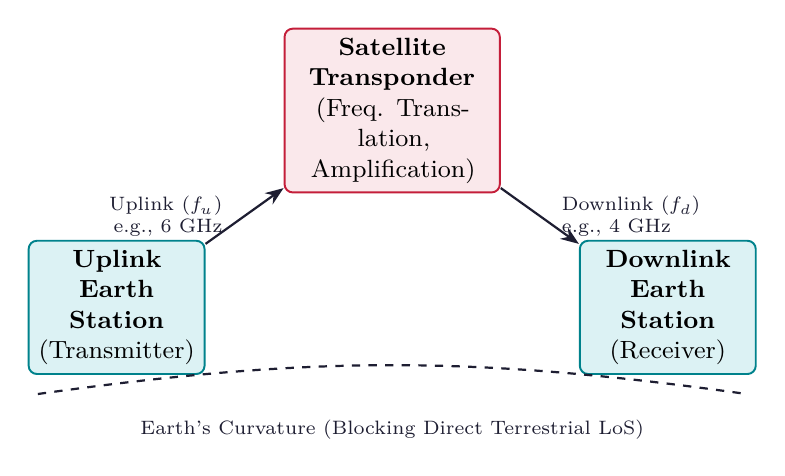
\begin{tikzpicture}[node distance=0.6cm and 1.2cm, every node/.style={font=\scriptsize}]
  % Ground Station Left
  \node[block, text width=2.0cm] (tx) at (0,0) {\textbf{Uplink Earth Station}\\(Transmitter)};
  
  % Satellite Node (Top Center)
  \node[redblock, text width=2.5cm] (sat) at (3.5,2.5) {\textbf{Satellite Transponder}\\(Freq. Translation,\\Amplification)};
  
  % Ground Station Right
  \node[block, text width=2.0cm] (rx) at (7.0,0) {\textbf{Downlink Earth Station}\\(Receiver)};
  
  % Arrows with frequency labels
  \draw[arrow] (tx) -- node[midway, left=0.15cm, align=right] {Uplink ($f_u$)\\e.g., 6 GHz} (sat);
  \draw[arrow] (sat) -- node[midway, right=0.15cm, align=left] {Downlink ($f_d$)\\e.g., 4 GHz} (rx);
  
  % Earth surface curve
  \draw[thick, color=mydark, dashed] (-1.0,-1.1) to[out=8, in=172] (8.0,-1.1);
  \node[below, align=center, color=mydark] at (3.5,-1.3) {Earth's Curvature (Blocking Direct Terrestrial LoS)};
\end{tikzpicture}
\end{tcolorbox}

% ===============================================================================
\section{Brief History of Satellite Systems}
% ===============================================================================

The theoretical concept of satellite communication was popularized by Arthur C. Clarke in 1945, who proposed using three geostationary satellites separated by $120^\circ$ to cover the entire globe. The operational milestones of satellite communication are outlined below:

\begin{itemize}[leftmargin=*, itemsep=3pt]
  \item \textbf{Sputnik 1 (1957):} Launched by the Soviet Union. It was the first artificial satellite in orbit, transmitting radio telemetry beeps at 20 MHz and 40 MHz.
  \item \textbf{Project Score (1958):} The first voice transmission satellite, launched by the United States. It broadcasted a pre-recorded Christmas message.
  \item \textbf{Echo 1 (1960):} A passive reflector balloon satellite that simply bounced radio signals off its metallized surface.
  \item \textbf{Telstar 1 (1962):} The first active, direct-amplifying communication satellite. It successfully transmitted live transatlantic television signals.
  \item \textbf{Syncom 3 (1964):} The first geostationary (GEO) communication satellite, which was used to broadcast the 1964 Tokyo Olympics.
  \item \textbf{Intelsat I (Early Bird, 1965):} The first commercial communications satellite, establishing regular telephone and TV traffic.
\end{itemize}

% ===============================================================================
\section{Advantages and Disadvantages of Satellite Communication}
% ===============================================================================

\textbf{Advantages:}
\begin{itemize}[leftmargin=*, itemsep=3pt]
  \item \textbf{Geographical Coverage:} A single geostationary satellite can cover up to 42.4\% of the Earth's surface. Only three satellites can cover the entire Earth (excluding polar regions).
  \item \textbf{Point-to-Multipoint Capability:} Ideal for broadcasting signals (e.g., satellite television) simultaneously to millions of receiving Earth terminals.
  \item \textbf{Independent of Terrestrial Infrastructure:} Highly reliable for emergency communications in rugged terrains, oceans, or disaster-struck areas where ground cables are non-existent or destroyed.
  \item \textbf{High Bandwidth:} Operates at high frequencies, providing large data capacity for television channels and broadband.
\end{itemize}

\textbf{Disadvantages:}
\begin{itemize}[leftmargin=*, itemsep=3pt]
  \item \textbf{Propagation Delay (Latency):} In Geostationary Earth Orbit (GEO), the round-trip distance is approximately 72,000 km, leading to a signal propagation latency of about 240 ms to 280 ms.
  \item \textbf{High Launch and Development Cost:} Designing, launching, and maintaining satellites in orbit requires massive capital investment and carries risks of launch failure.
  \item \textbf{No Servicing or Maintenance:} Once launched, satellites are generally impossible to service physically. Any hardware failure can render the entire system useless.
  \item \textbf{Vulnerability to Interference:} Subject to solar eclipse outages, atmospheric absorption, and radio frequency interference (RFI) from other terrestrial transmitters.
\end{itemize}

% ===============================================================================
\section{Applications of Satellite Communication}
% ===============================================================================

Satellite systems have permeated both civilian and military domains due to their global reach:

\begin{enumerate}[label=\textbf{\arabic*.}, leftmargin=*, itemsep=4pt]
  \item \textbf{Broadcast Television and Radio:} Direct-to-Home (DTH) satellite TV transmits digital programming directly to household dish antennas.
  \item \textbf{Satellite Telephony and Internet:} Inmarsat, Iridium, and Starlink systems provide satellite broadband and voice calls in remote, maritime, and aeronautical zones.
  \item \textbf{Global Navigation Satellite Systems (GNSS):} Systems like GPS (US), GLONASS (Russia), Galileo (EU), and NavIC (India) use orbital constellations to provide precise 3D positioning and timing.
  \item \textbf{Meteorology and Earth Observation:} Satellites track weather systems, hurricane paths, ocean temperatures, and environmental changes.
  \item \textbf{Military Reconnaissance and Tactical Comms:} Encrypted tactical communication links, troop tracking, drone navigation, and ballistic missile early warning networks.
\end{enumerate}

% ===============================================================================
\section{Frequency Bands Used for Satellite Communication}
% ===============================================================================

The International Telecommunication Union (ITU) regulates the allocation of frequencies to prevent mutual interference. Satellite links operate in microwave frequencies, allowing them to penetrate the Earth's ionosphere.

\subsection{Standard Frequency Band Classification}
The table below details the frequency bands used for satellite links:

\par\noindent
{\renewcommand{\arraystretch}{1.55}%
\begin{tabularx}{\linewidth}{|B{2.2cm}|>{\centering\arraybackslash}m{2.5cm}|>{\centering\arraybackslash}m{2.5cm}|Y|}\hline
\textbf{Band} & \textbf{Uplink Range} & \textbf{Downlink Range} & \textbf{Key Advantages / Applications} \\[4pt]
\hline
\textbf{L Band} & $1.61 - 1.66$ GHz & $1.52 - 1.56$ GHz & Low attenuation, small antennas; GPS, mobile satellite terminals (Iridium). \\[4pt]
\hline
\textbf{S Band} & $2.1 - 2.3$ GHz & $1.9 - 2.1$ GHz & Minimal rain fade; Mobile satellite service, DTH audio broadcasting. \\[4pt]
\hline
\textbf{C Band} & $5.92 - 6.42$ GHz & $3.7 - 4.2$ GHz & Highly mature technology, low rain fade; Telephony, TV networks, VSAT systems. \\[4pt]
\hline
\textbf{X Band} & $7.9 - 8.4$ GHz & $7.25 - 7.75$ GHz & Highly secure, military exclusive; Reconnaissance, military communications. \\[4pt]
\hline
\textbf{Ku Band} & $14.0 - 14.5$ GHz & $11.7 - 12.2$ GHz & High gain, smaller dish size; DTH TV, VSAT networks, high-speed data. \\[4pt]
\hline
\textbf{Ka Band} & $27.5 - 31.0$ GHz & $17.7 - 21.2$ GHz & Massive bandwidth; Satellite broadband (Starlink, Viasat), high-throughput systems. \\[4pt]
\hline
\end{tabularx}
}

\subsection{Uplink vs. Downlink Frequency Separation}
In satellite systems, the uplink frequency ($f_u$) is \textbf{always higher} than the downlink frequency ($f_d$).
\begin{equation}
  f_u > f_d
\end{equation}
This design choice is guided by three main engineering reasons:
\begin{enumerate}[label=\textbf{\alph*.}, leftmargin=*, itemsep=2pt]
  \item \textbf{Atmospheric Loss Compensation:} Propagation attenuation (such as rain fade) increases with frequency. An Earth station has access to high-power grid electricity, allowing it to easily output high power to overcome these losses at higher uplink frequencies. The satellite, however, has a limited power budget (relying on solar panels and batteries) and must use the lower, less attenuated frequency ($f_d$) for its downlink broadcast to conserve power.
  \item \textbf{Antenna Gain and Size:} High frequencies yield smaller wavelengths ($\lambda$), allowing the Earth station to achieve a narrower, more focused uplink beam with a reasonably sized dish.
  \item \textbf{Feedback Prevention:} The frequency translation prevents electromagnetic feedback loop oscillations inside the satellite transponder.
\end{enumerate}

% ===============================================================================
% MANDATORY QUICK REVISION PAGE
% ===============================================================================
\newpage
\begin{center}
  {\large\bfseries\color{myred} Quick Revision --- Module I}\\[3pt]
  {\small\color{mydark} Introduction to Satellite Communication $|$ PE-EC701B}
\end{center}
\noindent{\color{myred}\rule{\linewidth}{1.2pt}}
\vspace{4pt}

\begin{tcolorbox}[formulabox, title={\textbf{Key Formulas at a Glance}}]
\renewcommand{\arraystretch}{1.3}
\begin{tabularx}{\linewidth}{B{4.5cm} X}Wavelength-Frequency & $\lambda = \frac{c}{f}$ \quad ($c \approx 3 \times 10^8$ m/s) \\[6pt]
One-Way Latency & $t = \frac{d}{c}$ \quad ($d \approx 35,786$ km for GEO) \\[6pt]
Round-Trip Delay & $T_d = 2 \times \frac{d}{c} \approx 238 \text{ ms}$ (minimum orbital path) \\[6pt]
Uplink vs Downlink & $f_{\text{uplink}} > f_{\text{downlink}}$ \quad (e.g., $6/4$ GHz for C-band, $14/12$ GHz for Ku-band)
\end{tabularx}
\end{tcolorbox}

\begin{tcolorbox}[defbox, title={\textbf{One-Line Definitions}}]
\begin{itemize}[leftmargin=*, itemsep=2.5pt, topsep=0pt]
  \item \textbf{Satellite communication:} Orbiting radio transponders routing signals between distant Earth stations.
  \item \textbf{Transponder:} Spacecraft equipment that receives, converts, and transmits RF carriers.
  \item \textbf{Uplink:} The radio link transmitting from Earth stations to the satellite.
  \item \textbf{Downlink:} The radio link transmitting from the satellite to Earth stations.
  \item \textbf{Frequency Translation:} Conversion of uplink frequency to downlink frequency to avoid feedback.
  \item \textbf{Rain Fade:} Attenuation of microwave signals due to scattering and absorption by rain droplets.
  \item \textbf{GEO:} Geostationary Earth Orbit, located at an altitude of approximately 35,786 km.
\end{itemize}
\end{tcolorbox}

\begin{tcolorbox}[exambox, title={\textbf{Frequently Asked / Viva Questions}}]
\begin{enumerate}[topsep=0pt, label=\textbf{Q\arabic*.}, itemsep=5pt]
  \item \Q{State the fundamental principle of satellite communication.}
    It operates as a line-of-sight microwave link using an active orbiting transponder to receive, translate, and retransmit signals across massive global distances.
  \item \Q{Why is the uplink frequency always higher than the downlink frequency ($f_u > f_d$)?}
    Earth stations have abundant power to transmit at higher frequencies which suffer more atmospheric loss, whereas satellites have constrained onboard power and must transmit down at lower, less attenuated frequencies.
  \item \Q{Who first conceptualized global satellite communication using geostationary orbits?}
    Arthur C. Clarke, in a 1945 paper titled "Extra-Terrestrial Relays", proposing three GEO satellites.
  \item \Q{What is the function of a transponder on a satellite?}
    To receive the uplink signal, filter out noise, down-convert the frequency to the downlink band, and amplify it for retransmission.
  \item \Q{List standard frequency band designations and their typical frequencies.}
    C-band ($6/4$ GHz), Ku-band ($14/12$ GHz), Ka-band ($30/20$ GHz), and S-band ($2$ GHz).
  \item \Q{What are the main advantages of satellite communication over terrestrial networks?}
    Vast geographical coverage (up to 42.4\% per GEO satellite), point-to-multipoint broadcasting, and independent operational viability in remote/disaster areas.
  \item \Q{Explain the propagation delay disadvantage of GEO satellites.}
    Due to the high altitude (35,786 km), signals travel at the speed of light, yielding a round-trip Earth-satellite-Earth latency of approximately 240 ms to 280 ms.
  \item \Q{What was Sputnik 1?}
    The first artificial satellite, launched by the USSR in October 1957, transmitting simple telemetry beeps.
  \item \Q{What is rain fade, and in which frequency bands is it most prominent?}
    It is signal attenuation caused by rain droplets. It is highly prominent at frequencies above 10 GHz (Ku and Ka bands).
  \item \Q{What is GPS, and what are its orbital parameters?}
    Global Positioning System, a medium Earth orbit (MEO) constellation orbiting at an altitude of ~20,200 km, providing precise navigation.
  \item \Q{How many satellites are required for global coverage, and why?}
    Three geostationary satellites separated by $120^\circ$ of longitude because each satellite covers approximately 42.4\% of the Earth's surface.
  \item \Q{What is the difference between active and passive satellites?}
    Passive satellites (like Echo 1) only reflect signals. Active satellites (like Telstar 1) amplify and process signals.
\end{enumerate}
\tcbset{colbacktitle=myteal, coltitle=white}
\end{tcolorbox}

\begin{tcolorbox}[tikzbox, title={Comparison of Satellite Frequency Bands}]
\renewcommand{\arraystretch}{1.4}
\par\noindent
{\renewcommand{\arraystretch}{1.55}%
\begin{tabularx}{\linewidth}{|B{2.5cm}|Y|Y|Y|}\hline
\textbf{Parameter} & \textbf{\color{myteal}C Band} & \textbf{\color{myred}Ku Band} & \textbf{\color{myamber}Ka Band} \\[4pt]
\hline
\textbf{Frequency (U/D)} & $6 / 4$ GHz & $14 / 12$ GHz & $30 / 20$ GHz \\
\hline
\textbf{Rain Fade} & Negligible / Low & Moderate & Very High \\
\hline
\textbf{Dish Antenna Size} & Large ($2.4 - 3.7$ m) & Small ($0.6 - 1.2$ m) & Very Small ($0.3 - 0.75$ m) \\[4pt]
\hline
\textbf{Applications} & Backhaul telephony, TV distribution, maritime links. & DTH satellite TV, home VSAT terminals. & Satellite broadband, high-throughput commercial services. \\[4pt]
\hline
\end{tabularx}
}
\end{tcolorbox}


% -- Module 2 -----------------------------------------------------------------
\modulestart{2}{Kepler's Laws of Planetary Motion}

\section{Kepler's Laws of Planetary Motion}
% ===============================================================================

Orbital mechanics is governed by Newton's laws of motion and gravitation, which validate Kepler's three empirical laws of planetary motion. Originally formulated for planets orbiting the Sun, they apply identically to artificial satellites orbiting the Earth.

\begin{tcolorbox}[defbox]
\textbf{Kepler's Laws:} Three laws describing the motion of orbiting bodies:
\begin{enumerate}[label=\textbf{\arabic*.}, leftmargin=*, noitemsep, topsep=2pt]
  \item Orbiting bodies travel in elliptical paths with the primary body at one focus.
  \item A line joining a satellite and its primary sweeps out equal areas in equal intervals of time.
  \item The square of the orbital period is proportional to the cube of the semimajor axis.
\end{enumerate}
\end{tcolorbox}

\subsection{First Law: Law of Ellipses}
The orbit of any satellite is an ellipse with the Earth at one of the two foci. An ellipse is defined by its semimajor axis $a$, semiminor axis $b$, and eccentricity $e$, which represents the deviation from a perfect circle:
\begin{equation}
  e = \frac{\sqrt{a^2 - b^2}}{a}
\end{equation}
For a circular orbit, $e = 0$. For an elliptical orbit, $0 < e < 1$.

\subsection{Second Law: Law of Equal Areas}
For equal time intervals ($t_2 - t_1 = t_4 - t_3$), the shaded area $A_{12}$ swept out by the orbital radius vector is equal to area $A_{34}$. This implies that the satellite's orbital speed is not constant:
\begin{itemize}[leftmargin=*, noitemsep]
  \item It travels fastest at \textbf{Perigee} (closest to Earth).
  \item It travels slowest at \textbf{Apogee} (farthest from Earth).
\end{itemize}

\subsection{Third Law: Harmonic Law}
The square of the orbital period ($T$) of a satellite is directly proportional to the cube of its semimajor axis ($a$):
\begin{equation}
  T^2 = \frac{4\pi^2 a^3}{\mu}
\end{equation}
Where:
\begin{itemize}[leftmargin=*, label=$\bullet$, noitemsep]
  \item $T$ = Orbital period (seconds, s)
  \item $a$ = Semimajor axis of the ellipse (meters, m)
  \item $\mu = G \cdot M_E \approx 3.986 \times 10^{14} \text{ m}^3/\text{s}^2$ (Earth's geocentric gravitational constant)
  \item $G = 6.674 \times 10^{-11} \text{ N}\cdot\text{m}^2/\text{kg}^2$ (Universal gravitational constant)
  \item $M_E \approx 5.972 \times 10^{24} \text{ kg}$ (Mass of the Earth)
\end{itemize}

% ===============================================================================
\section{Elliptical Orbit Geometry: Apogee and Perigee}
% ===============================================================================

An elliptical orbit is characterized by its points of minimum and maximum distance from the Earth's center of mass.

\begin{tcolorbox}[tikzbox, title={Elliptical Orbit Geometry with Earth at Focus}]
\centering
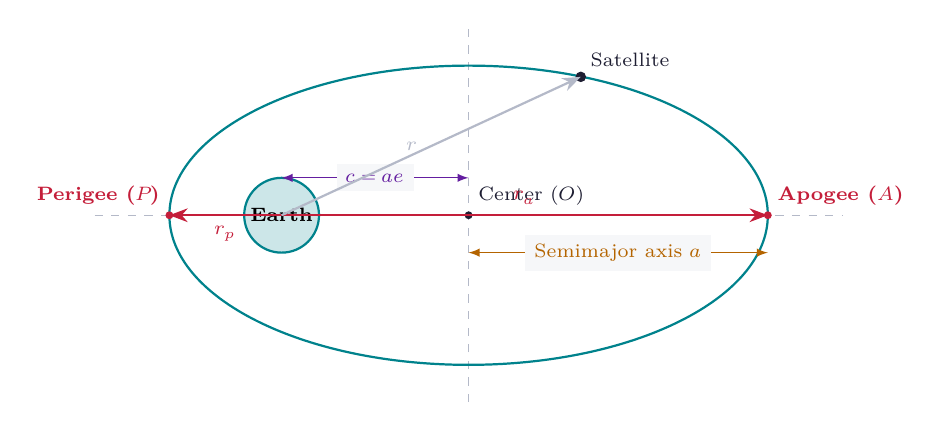
\begin{tikzpicture}[scale=0.95, every node/.style={font=\scriptsize}]
  % Draw axes
  \draw[dashed, color=mgframe] (-5.0,0) -- (5.0,0);
  \draw[dashed, color=mgframe] (0,-2.5) -- (0,2.5);
  
  % Draw Ellipse
  \draw[thick, color=myteal] (0,0) ellipse (4.0cm and 2.0cm);
  
  % Foci points
  \coordinate (F1) at (-2.5, 0); % Earth focus
  \coordinate (F2) at (2.5, 0);
  
  % Draw Earth at F1
  \fill[color=myteal!20, draw=myteal, line width=0.8pt] (F1) circle (0.5cm);
  \node at (F1) {\textbf{Earth}};
  
  % Center marker
  \fill[color=mydark] (0,0) circle (1.5pt) node[above right] {Center ($O$)};
  
  % Perigee and Apogee points
  \fill[color=myred] (-4.0,0) circle (1.5pt) node[above left, color=myred] {\textbf{Perigee ($P$)}};
  \fill[color=myred] (4.0,0) circle (1.5pt) node[above right, color=myred] {\textbf{Apogee ($A$)}};
  
  % Dimension lines
  % Semimajor axis 'a'
  \draw[latex-latex, color=myamber] (0,-0.5) -- node[midway, fill=mygray] {Semimajor axis $a$} (4.0,-0.5);
  % Focus distance 'ae'
  \draw[latex-latex, color=mypurple] (-2.5,0.5) -- node[midway, fill=mygray] {$c = ae$} (0,0.5);
  
  % Radius vectors
  \draw[arrow, color=myred] (F1) -- node[midway, below] {$r_p$} (-4.0,0);
  \draw[arrow, color=myred] (F1) -- node[midway, above] {$r_a$} (4.0,0);
  
  % Satellite on orbit
  \coordinate (Sat) at (1.5, 1.85);
  \fill[color=mydark] (Sat) circle (2pt) node[above right] {Satellite};
  \draw[arrow, color=mgframe] (F1) -- node[midway, left=0.05cm] {$r$} (Sat);
\end{tikzpicture}
\end{tcolorbox}

\subsection{Key Parameters and Formulas}
From the geometry of the ellipse:
\begin{enumerate}[label=\textbf{\arabic*.}, leftmargin=*, itemsep=3pt]
  \item \textbf{Perigee Distance ($r_p$):} The point of closest approach to the center of Earth.
    \begin{equation}
      r_p = a(1 - e)
    \end{equation}
  \item \textbf{Apogee Distance ($r_a$):} The point of farthest distance from the center of Earth.
    \begin{equation}
      r_a = a(1 + e)
    \end{equation}
  \item \textbf{Relationship to Altitudes:}
    \begin{equation}
      a = \frac{r_a + r_p}{2}
    \end{equation}
    \begin{equation}
      e = \frac{r_a - r_p}{r_a + r_p}
    \end{equation}
    Where $r_a = R_E + h_a$ and $r_p = R_E + h_p$ ($R_E \approx 6378 \text{ km}$ is Earth's mean radius, $h_a, h_p$ are apogee/perigee altitudes above Earth's surface).
\end{enumerate}

% ===============================================================================
\section{Orbital Equations and Parameters}
% ===============================================================================

The dynamics of a satellite are dictated by the balancing of gravitational and centripetal forces.

\subsection{Orbital Velocity}
The instantaneous velocity ($v$) of a satellite orbiting in an elliptical path at a distance $r$ from the center of Earth is given by the \textbf{Vis-Viva Equation}:
\begin{equation}
  v = \sqrt{\mu \left( \frac{2}{r} - \frac{1}{a} \right)}
\end{equation}

\begin{itemize}[leftmargin=*, itemsep=6pt]
  \item \textbf{For Circular Orbits ($r = a$):} The velocity remains constant at:
    \begin{equation}
      v_{c} = \sqrt{\frac{\mu}{r}}
    \end{equation}
  \item \textbf{At Perigee ($r = r_p = a(1-e)$):} The velocity is at its maximum:
    \begin{equation}
      v_{max} = \sqrt{\frac{\mu}{a}\left(\frac{1+e}{1-e}\right)}
    \end{equation}
  \item \textbf{At Apogee ($r = r_a = a(1+e)$):} The velocity is at its minimum:
    \begin{equation}
      v_{min} = \sqrt{\frac{\mu}{a}\left(\frac{1-e}{1+e}\right)}
    \end{equation}
\end{itemize}

\subsection{Angular Velocity}
The mean angular velocity ($\omega$) of a satellite in circular orbit (or the average mean motion $n$) is:
\begin{equation}
  \omega = \frac{2\pi}{T} = \sqrt{\frac{\mu}{a^3}}
\end{equation}
The instantaneous angular velocity at any distance $r$ is derived from conservation of angular momentum:
\begin{equation}
  \omega_{inst} = \frac{h}{r^2}
\end{equation}
Where $h = \sqrt{\mu a(1 - e^2)}$ is the specific angular momentum of the orbit.

% ===============================================================================
\section{Solar Day vs. Sidereal Day}
% ===============================================================================

To design satellite orbits that synchronize with Earth's rotation (like geostationary orbits), we must distinguish between two methods of measuring a day.

\begin{tcolorbox}[defbox]
\textbf{Solar Day:} The time taken for the Earth to rotate once about its axis relative to the Sun. It is exactly \textbf{24 hours} (86,400 seconds).

\textbf{Sidereal Day:} The time taken for the Earth to rotate once about its axis relative to the distant stars (inertial space). It is exactly \textbf{23 hours, 56 minutes, and 4.09 seconds} (86,164.09 seconds).
\end{tcolorbox}

\subsection{The Astronomical Difference}
Because the Earth orbits the Sun while rotating on its axis, it travels approximately $1^\circ$ along its orbital path each day. Consequently, the Earth must rotate slightly more than $360^\circ$ (about $360.986^\circ$) to bring the Sun back to the same meridian. A sidereal day is a true $360^\circ$ rotation.

\begin{tcolorbox}[tikzbox, title={Earth Rotation: Solar Day vs. Sidereal Day}]
\centering
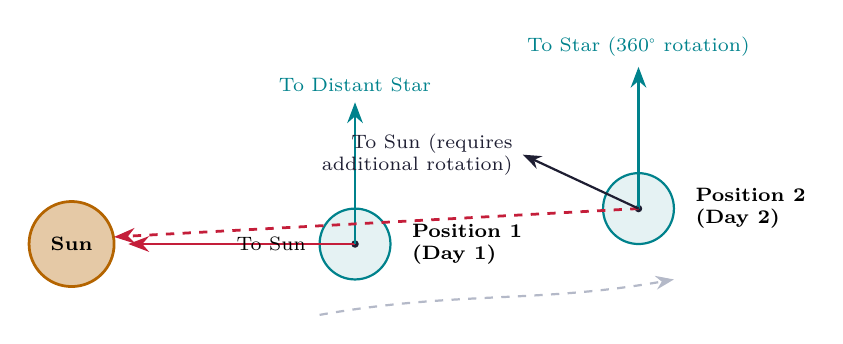
\begin{tikzpicture}[scale=0.9, every node/.style={font=\scriptsize}]
  % Sun (Left side)
  \fill[color=myamber!35, draw=myamber, line width=1.0pt] (-4,0) circle (0.6cm);
  \node at (-4,0) {\textbf{Sun}};
  
  % Earth Position 1 (Day 1)
  \coordinate (E1) at (0,0);
  \draw[thick, fill=myteal!10, draw=myteal] (E1) circle (0.5cm);
  \fill[color=mydark] (E1) circle (1.5pt);
  \node[right=0.6cm of E1, align=left] {\textbf{Position 1}\\\textbf{(Day 1)}};
  
  % Pointing vector to Sun and Star
  \draw[arrow, color=myred, line width=1pt] (E1) -- (-3.2,0);
  \draw[arrow, color=myteal, line width=1pt] (E1) -- (0,2) node[above] {To Distant Star};
  \node[left=0.5cm of E1] {To Sun};
  
  % Earth Position 2 (Day 2) after 360 rotation (Sidereal Day complete)
  \coordinate (E2) at (4,0.5);
  \draw[thick, fill=myteal!10, draw=myteal] (E2) circle (0.5cm);
  \fill[color=mydark] (E2) circle (1.5pt);
  \node[right=0.6cm of E2, align=left] {\textbf{Position 2}\\\textbf{(Day 2)}};
  
  % Pointing vectors at Position 2
  \draw[arrow, color=myteal, line width=1pt] (E2) -- (4,2.5) node[above] {To Star ($360^\circ$ rotation)};
  \draw[arrow, color=myred, line width=1pt, dashed] (E2) -- (-3.4,0.1); % Pointing to Sun
  \draw[arrow, color=mydark, line width=0.8pt] (E2) -- ($(E2)+(155:1.8)$) node[left, align=right] {To Sun (requires\\additional rotation)};
  
  % Orbit path
  \draw[arrow, dashed, color=mgframe] (-0.5,-1) to[out=10, in=190] (4.5,-0.5);
\end{tikzpicture}
\end{tcolorbox}

\subsection{Impact on Geostationary Orbit (GEO) Design}
A geostationary satellite must remain fixed relative to a point on the Earth. Therefore, its orbital period must match the Earth's inertial rotation rate, which is the \textbf{sidereal day} ($T = 86,164.09$ seconds), rather than the solar day.

Substituting $T = 86,164.09$ s into Kepler's Third Law:
\begin{equation}
  a^3 = \frac{T^2 \mu}{4\pi^2} = \frac{(86,164.09)^2 \times 3.986 \times 10^{14}}{4\pi^2} \approx 7.496 \times 10^{22} \text{ m}^3
\end{equation}
\begin{equation}
  a \approx 42,164 \text{ km}
\end{equation}
Subtracting Earth's equatorial radius ($R_E \approx 6,378$ km):
\begin{equation}
  h_{GEO} = a - R_E \approx 35,786 \text{ km}
\end{equation}
This derivation establishes the standard altitude of geostationary satellites.

% ===============================================================================
% MANDATORY QUICK REVISION PAGE
% ===============================================================================
\newpage
\begin{center}
  {\large\bfseries\color{myred} Quick Revision --- Module II}\\[3pt]
  {\small\color{mydark} Orbital Mechanics $|$ PE-EC701B}
\end{center}
\noindent{\color{myred}\rule{\linewidth}{1.2pt}}
\vspace{4pt}

\begin{tcolorbox}[formulabox, title={\textbf{Key Formulas at a Glance}}]
\renewcommand{\arraystretch}{1.9}
\begin{tabularx}{\linewidth}{B{5.0cm} X}Kepler's Third Law & $\displaystyle T^2 = \frac{4\pi^2 a^3}{\mu}$ \quad ($\mu \approx 3.986 \times 10^{14} \text{ m}^3/\text{s}^2$) \\[4pt]
Vis-Viva (Velocity) Equation & $\displaystyle v = \sqrt{\mu\left(\frac{2}{r} - \frac{1}{a}\right)}$ \\[4pt]
Apogee \& Perigee Distance & $r_a = a(1 + e)$ \quad and \quad $r_p = a(1 - e)$ \\[4pt]
Eccentricity from Radii & $\displaystyle e = \frac{r_a - r_p}{r_a + r_p} = \frac{\sqrt{a^2 - b^2}}{a}$ \\[4pt]
Mean Motion / Angular Velocity & $\displaystyle \omega = \sqrt{\frac{\mu}{a^3}}$
\end{tabularx}
\end{tcolorbox}

\begin{tcolorbox}[defbox, title={\textbf{One-Line Definitions}}]
\begin{itemize}[leftmargin=*, itemsep=2.5pt, topsep=0pt]
  \item \textbf{Apogee:} The point in an orbit farthest from the center of the Earth.
  \item \textbf{Perigee:} The point in an orbit closest to the center of the Earth.
  \item \textbf{Eccentricity:} A parameter determining how much an orbit deviates from a perfect circle.
  \item \textbf{Vis-Viva Equation:} The direct mathematical relationship for velocity at any orbital radius.
  \item \textbf{Sidereal Day:} Time for Earth to rotate $360^\circ$ relative to distant stars (86,164.09 s).
  \item \textbf{Solar Day:} Time for Earth to align back with the Sun (86,400 s).
  \item \textbf{Geocentric Constant ($\mu$):} Product of Gravitational Constant $G$ and Mass of Earth $M_E$.
\end{itemize}
\end{tcolorbox}

\begin{tcolorbox}[exambox, title={\textbf{Frequently Asked / Viva Questions}}]
\begin{enumerate}[topsep=0pt, label=\textbf{Q\arabic*.}, itemsep=5pt]
  \item \Q{State Kepler's Second Law and explain its velocity implication.}
    A line joining a satellite and its primary sweeps out equal areas in equal times. Thus, velocity is not constant; the satellite accelerates as it approaches perigee and decelerates as it approaches apogee.
  \item \Q{Derive the orbital radius of a geostationary satellite.}
    Using Kepler's 3rd Law ($T^2 = 4\pi^2 a^3/\mu$) and substituting the sidereal day ($T = 86,164$ s) and $\mu = 3.986 \times 10^5 \text{ km}^3/\text{s}^2$, we get $a \approx 42,164$ km. Subtracting $R_E \approx 6,378$ km yields $h \approx 35,786$ km.
  \item \Q{What is the difference between a sidereal day and a solar day?}
    A sidereal day is measured relative to distant stars ($23\text{h }56\text{m }4\text{s}$), whereas a solar day is measured relative to the Sun ($24\text{h}$). The difference arises because the Earth moves along its orbit around the Sun.
  \item \Q{Define eccentricity ($e$) and state its values for circular, elliptical, parabolic, and hyperbolic trajectories.}
    Eccentricity defines orbital shape. Circle: $e = 0$; Ellipse: $0 < e < 1$; Parabola: $e = 1$ (escape trajectory); Hyperbola: $e > 1$.
  \item \Q{Where is the satellite velocity maximum and minimum, and what are the expressions?}
    Maximum at perigee: $v_{max} = \sqrt{\frac{\mu}{a}\left(\frac{1+e}{1-e}\right)}$. Minimum at apogee: $v_{min} = \sqrt{\frac{\mu}{a}\left(\frac{1-e}{1+e}\right)}$.
  \item \Q{What is the physical significance of the geocentric gravitational constant ($\mu$)?}
    It is the product $G \cdot M_E$ (approx $3.986 \times 10^{14} \text{ m}^3/\text{s}^2$). It simplifies orbital math by combining the mass of the primary body and the gravitational constant.
  \item \Q{Why does a satellite not fall to Earth if gravity is constantly pulling it?}
    The satellite's high tangential velocity creates a centrifugal effect that balances the Earth's gravitational pull. It is in a continuous state of free fall around Earth's curve.
  \item \Q{An elliptical orbit has $r_p = 7,000$ km and $r_a = 15,000$ km. Calculate the semimajor axis and eccentricity.}
    $a = (r_a + r_p)/2 = 11,000$ km. $e = (r_a - r_p)/(r_a + r_p) = (15000-7000)/(15000+7000) = 8/22 \approx 0.364$.
  \item \Q{How does the orbital period change if the altitude of a satellite is doubled?}
    Since $T \propto a^{1.5}$, if $a$ increases, the period $T$ increases by $2^{1.5} \approx 2.83$ times.
  \item \Q{What is specific angular momentum ($h$) of an orbit?}
    It is the angular momentum per unit mass, $h = r \times v$. It remains constant along the orbit, demonstrating Kepler's second law.
  \item \Q{What is the escape velocity from Earth's surface?}
    $v_{esc} = \sqrt{2gR_E} = \sqrt{2\mu/R_E} \approx 11.2 \text{ km/s}$.
  \item \Q{How does body eccentricity impact solar day length?}
    If Earth's orbit eccentricity were larger, the orbital speed around the Sun would vary more, causing the solar day duration to fluctuate significantly throughout the year.
\end{enumerate}
\tcbset{colbacktitle=myteal, coltitle=white}
\end{tcolorbox}

\begin{tcolorbox}[tikzbox, title={Comparison of Earth Orbit Altitudes}]
\renewcommand{\arraystretch}{1.4}
\par\noindent
{\renewcommand{\arraystretch}{1.55}%
\begin{tabularx}{\linewidth}{|B{3.2cm}|Y|Y|Y|}\hline
\textbf{Orbit Class} & \textbf{Typical Altitude ($h$)} & \textbf{Orbital Period ($T$)} & \textbf{Primary Application} \\[4pt]
\hline
\textbf{LEO (Low Earth)} & $160 - 2,000$ km & $90 - 120$ minutes & Earth imaging, ISS, Starlink satellite constellations. \\[4pt]
\hline
\textbf{MEO (Medium Earth)} & $2,000 - 35,000$ km & $2 - 24$ hours & GPS (~12 hours), Galileo navigation constellations. \\[4pt]
\hline
\textbf{GEO (Geostationary)} & $35,786$ km & $23\text{h }56\text{m }4\text{s}$ (Sidereal) & Weather satellites, satellite TV broadcast, VSAT links. \\[4pt]
\hline
\textbf{HEO (Highly Elliptical)} & $1,000 - 40,000$ km (Molniya) & ~$12$ hours & Communication at high polar latitudes (Russian Molniya). \\[4pt]
\hline
\end{tabularx}
}
\end{tcolorbox}


% -- Module 3 -----------------------------------------------------------------
\modulestart{3}{Satellite Sub-systems Architecture}

\section{Satellite Sub-systems Architecture}
% ===============================================================================

A spacecraft consists of two primary operational components: the \textbf{Payload} (which performs the primary communication task) and the \textbf{Bus} (which provides the physical support infrastructure, power, stabilization, and control necessary for the payload to function).

\begin{tcolorbox}[defbox]
\textbf{Satellite Bus \& Payload:} The \textbf{payload} refers to the communication transponders and antennas. The \textbf{bus} refers to the physical support systems including the structural frame, thermal shielding, power generation, propulsion, stabilization (AOCS), and monitoring (TTC\&M).
\end{tcolorbox}

\subsection{Sub-systems Overview}
The subsystems must work in synchronization to maintain the satellite's health and functionality. The relationship between the systems is mapped below:

\begin{tcolorbox}[tikzbox, title={Satellite Sub-systems Integration}]
\centering
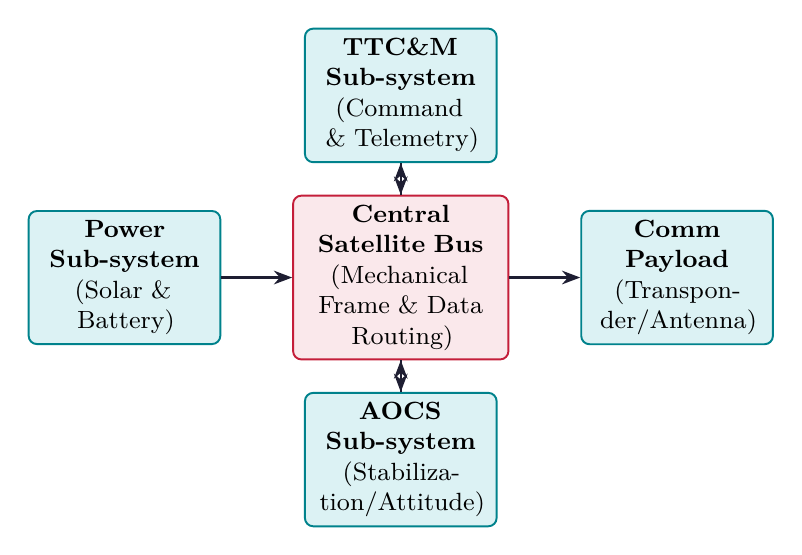
\begin{tikzpicture}[node distance=0.4cm and 0.9cm, every node/.style={font=\scriptsize}]
  % Central integration node
  \node[redblock, text width=2.5cm, minimum height=1.2cm] (bus) {\textbf{Central Satellite Bus}\\(Mechanical Frame \& Data Routing)};
  
  % Surrounding subsystems
  \node[block, above=of bus, text width=2.2cm] (ttcm) {\textbf{TTC\&M Sub-system}\\(Command \& Telemetry)};
  \node[block, below=of bus, text width=2.2cm] (aocs) {\textbf{AOCS Sub-system}\\(Stabilization/Attitude)};
  \node[block, left=of bus, text width=2.2cm] (power) {\textbf{Power Sub-system}\\(Solar \& Battery)};
  \node[block, right=of bus, text width=2.2cm] (payload) {\textbf{Comm Payload}\\(Transponder/Antenna)};
  
  % Interconnections
  \draw[arrow] (ttcm) -- (bus);
  \draw[arrow] (bus) -- (ttcm);
  \draw[arrow] (aocs) -- (bus);
  \draw[arrow] (bus) -- (aocs);
  \draw[arrow] (power) -- (bus);
  \draw[arrow] (bus) -- (payload);
\end{tikzpicture}
\end{tcolorbox}

% ===============================================================================
\section{Telemetry, Tracking, Command, and Monitoring (TTC\&M)}
% ===============================================================================

The TTC\&M sub-system establishes a constant bi-directional radio control link between the satellite and the ground control station (Earth Station).

\begin{itemize}[leftmargin=*, itemsep=3.5pt]
  \item \textbf{Telemetry (Transmission from Space to Earth):} Gathers diagnostic sensor data onboard the satellite (such as battery voltage, solar cell current, internal temperature, and gas pressure) and transmits this status information to Earth.
  \item \textbf{Tracking (Determination of Position):} Measures slant range, angular coordinates, and Doppler shift of the satellite's beacon to compute its precise orbital position, ensuring it has not drifted.
  \item \textbf{Command (Reception from Earth to Space):} Receives control instructions from the ground station to execute tasks like firing thrusters for orbital correction, switching transponder channels, or deploying solar arrays.
  \item \textbf{Monitoring:} Continuous checking of payload performance and checking for anomalies.
\end{itemize}

% ===============================================================================
\section{Attitude and Orbit Control System (AOCS)}
% ===============================================================================

The AOCS is responsible for keeping the satellite in its correct orbital slot (station-keeping) and ensuring its antennas and solar panels are pointing in the correct directions (attitude control).

\begin{itemize}[leftmargin=*, itemsep=4pt]
  \item \textbf{Attitude Control:} Stabilizes the satellite relative to its three axes:
    \begin{itemize}[leftmargin=*, itemsep=2pt, topsep=2pt]
      \item \textbf{Roll:} Rotation around the longitudinal axis (tangent to orbit velocity).
      \item \textbf{Pitch:} Rotation around the lateral axis (perpendicular to orbit plane).
      \item \textbf{Yaw:} Rotation around the vertical axis (pointing toward Earth's center).
    \end{itemize}
  \item \textbf{Orbit Control (Station Keeping):} Fires thrusters to correct long-term orbital drift caused by gravitational pulls from the Sun/Moon, Earth's equatorial asymmetry (ellipticity), and solar radiation pressure.
\end{itemize}

\subsection{Stabilization Techniques}
There are two main methods to keep a satellite from tumbling:
\begin{enumerate}[label=\textbf{\arabic*.}, leftmargin=*, itemsep=2pt]
  \item \textbf{Spin Stabilization:} The satellite body is spun rapidly at 30 to 100 rpm, using gyroscopic momentum to maintain axis alignment. The antennas must be mounted on a "despun" platform rotating in the opposite direction to remain fixed on Earth.
  \item \textbf{Three-Axis (Body) Stabilization:} The satellite body remains fixed relative to Earth. Momentum wheels or reaction wheels inside the satellite spin at varying speeds to absorb and counteract external disturbance torques.
\end{enumerate}

% ===============================================================================
\section{Communication Sub-system: Transponders}
% ===============================================================================

The transponder is the heart of the communication payload. A satellite typical houses 12 to 96 transponders, each acting as a separate channel.

\subsection{Bent-Pipe (Frequency Translation) Transponder}
Also known as a \textbf{repeater transponder}. It simply amplifies the incoming signal, down-converts its frequency, and transmits it. It does not look at or alter the digital content.

\begin{tcolorbox}[tikzbox, title={Bent-Pipe Transponder Block Diagram}]
\centering
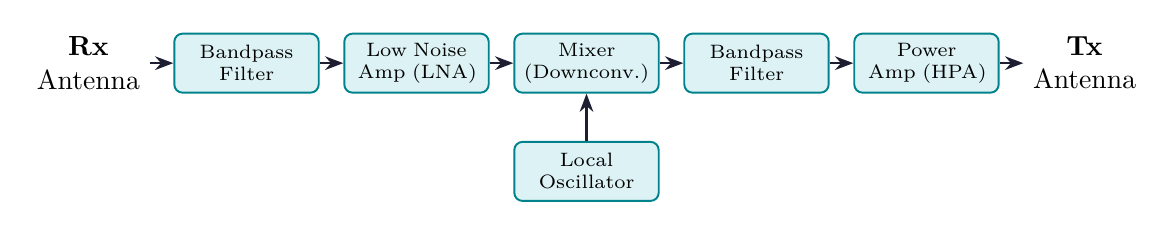
\begin{tikzpicture}[node distance=0.2cm and 0.4cm,
  sblock/.style={rectangle, draw=myteal, fill=hdrteal, text width=1.6cm,
    align=center, minimum height=0.75cm, font=\scriptsize,
    rounded corners=3pt, line width=0.7pt}]
  
  % Nodes
  \node (ant_rx) [align=center] {\textbf{Rx}\\Antenna};
  \node[sblock, right=0.3cm of ant_rx] (bpf1) {Bandpass\\Filter};
  \node[sblock, right=0.3cm of bpf1] (lna) {Low Noise\\Amp (LNA)};
  \node[sblock, right=0.3cm of lna] (mixer) {Mixer\\(Downconv.)};
  \node[sblock, below=0.6cm of mixer] (lo) {Local\\Oscillator};
  \node[sblock, right=0.3cm of mixer] (bpf2) {Bandpass\\Filter};
  \node[sblock, right=0.3cm of bpf2] (hpa) {Power\\Amp (HPA)};
  \node (ant_tx) [right=0.3cm of hpa, align=center] {\textbf{Tx}\\Antenna};
  
  % Arrows
  \draw[arrow] (ant_rx) -- (bpf1);
  \draw[arrow] (bpf1) -- (lna);
  \draw[arrow] (lna) -- (mixer);
  \draw[arrow] (lo) -- (mixer);
  \draw[arrow] (mixer) -- (bpf2);
  \draw[arrow] (bpf2) -- (hpa);
  \draw[arrow] (hpa) -- (ant_tx);
\end{tikzpicture}
\end{tcolorbox}

\begin{itemize}[leftmargin=*, itemsep=3.5pt]
  \item \textbf{Low Noise Amplifier (LNA):} Amplifies the extremely weak uplink signal (in the range of picowatts) while adding minimal thermal noise.
  \item \textbf{Mixer \& Local Oscillator:} Translates the signal frequency. The shift is $\Delta f = f_{LO} = f_u - f_d$ (e.g., $6 \text{ GHz} - 4 \text{ GHz} = 2 \text{ GHz}$).
  \item \textbf{High Power Amplifier (HPA):} Amplifies the downlink signal to several watts using Traveling-Wave Tube Amplifiers (TWTAs) or Solid-State Power Amplifiers (SSPAs) for transmission.
\end{itemize}

\subsection{Regenerative (Demodulation/Remodulation) Transponder}
A regenerative transponder demodulates the incoming analog signal down to the digital baseband bitstream, cleans up the digital noise (performing error correction), and then remodulates the digital data onto a new downlink carrier.
It acts as a \textbf{"computer in space"}, isolating the uplink noise from the downlink path.

% ===============================================================================
\section{Power Sub-system}
% ===============================================================================

The power subsystem must generate, store, regulate, and distribute electrical power.
\begin{itemize}[leftmargin=*, itemsep=3.5pt]
  \item \textbf{Primary Source (Solar Arrays):} Gallium Arsenide (GaAs) or Silicon solar panels convert solar energy into electrical power. In GEO, arrays must continuously track the Sun.
  \item \textbf{Secondary Source (Batteries):} Rechargeable batteries (Nickel-Hydrogen $\text{Ni-H}_2$ or Lithium-Ion) store electrical energy to power the spacecraft during \textbf{solar eclipses} when Earth blocks sunlight.
  \item \textbf{Power Conditioning Unit (PCU):} Regulates the bus voltage (typically 28V, 50V, or 100V DC) and controls battery charging/discharge rates.
\end{itemize}

% ===============================================================================
% MANDATORY QUICK REVISION PAGE
% ===============================================================================
\newpage
\begin{center}
  {\large\bfseries\color{myred} Quick Revision --- Module III}\\[3pt]
  {\small\color{mydark} Satellite Sub-systems $|$ PE-EC701B}
\end{center}
\noindent{\color{myred}\rule{\linewidth}{1.2pt}}
\vspace{4pt}

\begin{tcolorbox}[formulabox, title={\textbf{Key Formulas at a Glance}}]
\renewcommand{\arraystretch}{1.3}
\begin{tabularx}{\linewidth}{B{5.0cm} X}LO Frequency Shift & $f_{LO} = f_{uplink} - f_{downlink}$ \\[4pt]
Solar Panel Efficiency & $P = \eta \cdot S \cdot A \cdot \cos(\theta)$ \quad ($S \approx 1367 \text{ W/m}^2$, $\eta$ = efficiency) \\[4pt]
Battery Capacity & $C_{req} = \frac{P_{load} \times t_{eclipse}}{DoD \times V_{bus}}$ \quad ($DoD$ = Depth of Discharge) \\[4pt]
Local Oscillator Shift (C-Band) & $f_{LO} = 5.925\text{ GHz} - 3.7\text{ GHz} = 2.225\text{ GHz}$
\end{tabularx}
\tcbset{colbacktitle=myteal, coltitle=white}
\end{tcolorbox}

\begin{tcolorbox}[defbox, title={\textbf{One-Line Definitions}}]
\begin{itemize}[leftmargin=*, itemsep=2.5pt, topsep=0pt]
  \item \textbf{TTC\&M:} Ground station radio link monitoring health, status, and position of the satellite.
  \item \textbf{AOCS:} The subsystem stabilizing satellite orientation and correcting orbital drift.
  \item \textbf{Bent-Pipe Transponder:} A simple frequency translation and amplification transponder.
  \item \textbf{Regenerative Transponder:} A transponder that demodulates, processes, and remodulates data.
  \item \textbf{Despun Platform:} A platform rotating oppositely to a spin-stabilized satellite body to keep antennas fixed.
  \item \textbf{Reaction Wheels:} Internal motor-driven wheels adjusting satellite attitude via conservation of angular momentum.
  \item \textbf{Station Keeping:} Maneuvers using thrusters to keep a satellite within its assigned orbital box.
\end{itemize}
\end{tcolorbox}

\begin{tcolorbox}[exambox, title={\textbf{Frequently Asked / Viva Questions}}]
\begin{enumerate}[topsep=0pt, label=\textbf{Q\arabic*.}, itemsep=5pt]
  \item \Q{Differentiate between satellite payload and satellite bus.}
    The payload represents the hardware performing the actual service (transponders and antennas). The bus represents the supporting infrastructure (structure, power, thermal, AOCS, TTC\&M).
  \item \Q{What are the functions of Telemetry and Command in TTC\&M?}
    Telemetry transmits internal sensor readings (health data) from the satellite to Earth. Command receives control signals from Earth to execute adjustments inside the satellite.
  \item \Q{Explain the three attitude axes of a satellite: Roll, Pitch, and Yaw.}
    Roll: rotation about the velocity vector. Pitch: rotation perpendicular to the orbit plane. Yaw: rotation pointing directly toward the center of the Earth.
  \item \Q{Compare Spin Stabilization and Three-Axis Stabilization.}
    Spin stabilization uses gyroscopic spin of the entire body to maintain axis alignment. Three-axis stabilization keeps the outer body stationary while internal reaction wheels spin dynamically to absorb disturbance torques.
  \item \Q{Draw the basic block diagram of a bent-pipe transponder.}
    Rx Antenna $\to$ BPF $\to$ LNA $\to$ Mixer (with LO) $\to$ BPF $\to$ HPA $\to$ Tx Antenna.
  \item \Q{Why is an LNA placed as the first block in the transponder receiver chain?}
    Because the received uplink signal is extremely weak. Amplifying it first with a Low Noise Amplifier establishes a high signal-to-noise ratio, preventing subsequent stages from corrupting the signal.
  \item \Q{What is the advantage of a regenerative transponder over a bent-pipe transponder?}
    It demodulates and decodes the signal, stripping away uplink noise and distortion. It then regenerates and remodulates the clean digital bits, preventing noise accumulation.
  \item \Q{Why do satellites require battery systems if they have solar panels?}
    Because satellites periodically pass through the Earth's shadow (solar eclipses) where solar panels cannot generate power. Batteries provide secondary power during these shadow periods.
  \item \Q{What is the function of the thrusters in the propulsion system?}
    To perform station-keeping (correcting orbital drift caused by Sun/Moon gravity) and attitude adjustments when reaction wheels saturate.
  \item \Q{What is Depth of Discharge (DoD) in satellite batteries?}
    It is the percentage of battery capacity used during an eclipse. Satellites restrict DoD to 50--80\% to maximize the operational lifespan of the batteries.
  \item \Q{Why is thermal control critical in spacecraft design?}
    In vacuum, heat is only transferred by radiation. The side facing the Sun heats to $>100^\circ\text{C}$ while the shadow side drops to $<-100^\circ\text{C}$. The thermal system redistributes heat to keep electronics in operational ranges.
  \item \Q{What is a local oscillator frequency offset, and how is it chosen?}
    It is chosen to match the frequency separation between uplink and downlink bands (e.g., 2.225 GHz offset for C-band) to prevent electromagnetic feedback.
\end{enumerate}
\end{tcolorbox}

\begin{tcolorbox}[tikzbox, title={Comparison of Transponder Architectures}]
\renewcommand{\arraystretch}{1.4}
\par\noindent
{\renewcommand{\arraystretch}{1.55}%
\begin{tabularx}{\linewidth}{|B{3.2cm}|Y|Y|}\hline
\textbf{Feature} & \textbf{\color{myteal}Bent-Pipe Transponder} & \textbf{\color{mypurple}Regenerative Transponder} \\[4pt]
\hline
\textbf{Basic Operation} & RF-to-RF translation & Demodulation $\to$ Baseband Processing $\to$ Remodulation \\[4pt]
\hline
\textbf{Noise Propagation} & Uplink noise is amplified and sent down. & Uplink noise is removed at baseband. \\[4pt]
\hline
\textbf{Complexity \& Weight} & Low complexity, lightweight, highly reliable. & High complexity, heavy, requires onboard processors. \\[4pt]
\hline
\textbf{Flexibility} & Protocol transparent (handles any modulation format). & Protocol-specific (locked to a particular modulation/coding standard). \\[4pt]
\hline
\textbf{Primary Use Case} & Standard satellite TV distribution, VSAT links. & Modern satellite broadband, military secure links. \\[4pt]
\hline
\end{tabularx}
}
\end{tcolorbox}


% -- Module 4 -----------------------------------------------------------------
\modulestart{4}{Solar Eclipse on Satellite}

\section{Solar Eclipse on Satellite}
% ===============================================================================

An orbital eclipse occurs when a satellite passes through the shadow cast by the Earth (or occasionally the Moon), blocking its direct line of sight to the Sun.

\begin{tcolorbox}[defbox]
\textbf{Solar Eclipse:} The condition where Earth's shadow blocks sunlight from reaching the satellite's solar panels. For geostationary (GEO) satellites, eclipses occur twice a year during the vernal and autumnal equinoxes for a 72-day period.
\end{tcolorbox}

\subsection{Eclipse Geometry and Occurrence}
Because the Earth's axis of rotation is tilted at $23.4^\circ$, GEO satellites bypass Earth's shadow during most of the year. However, during the equinoxes (late March and late September), the Sun lies in the Earth's equatorial plane, aligning the Sun, Earth, and GEO satellites.

\begin{tcolorbox}[tikzbox, title={GEO Satellite Solar Eclipse Geometry}]
\centering
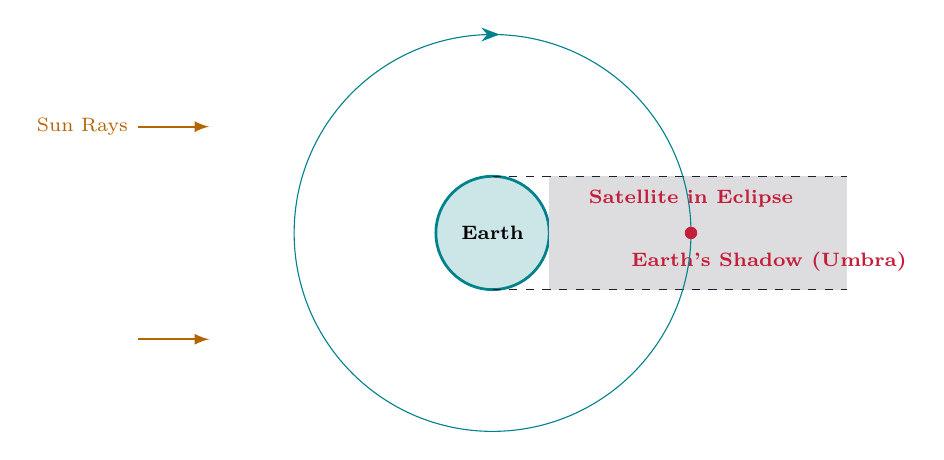
\begin{tikzpicture}[scale=0.9, every node/.style={font=\scriptsize}]
  % Sun rays (left side)
  \draw[latex-, color=myamber, thick] (-4,1.5) -- (-5,1.5) node[left] {Sun Rays};
  \draw[latex-, color=myamber, thick] (-4,-1.5) -- (-5,-1.5);
  
  % Earth (Center)
  \fill[color=myteal!20, draw=myteal, line width=1pt] (0,0) circle (0.8cm);
  \node at (0,0) {\textbf{Earth}};
  
  % Shadow boundaries (Umbra)
  \fill[color=mydark!15] (0.8,0.8) -- (5.0,0.8) -- (5.0,-0.8) -- (0.8,-0.8) -- cycle;
  \draw[dashed, color=mydark] (0,0.8) -- (5.0,0.8);
  \draw[dashed, color=mydark] (0,-0.8) -- (5.0,-0.8);
  \node[color=myred] at (3.9,-0.4) {\textbf{Earth's Shadow (Umbra)}};
  
  % Satellite Orbit Path
  \draw[color=myteal, thin] (0,0) circle (2.8cm);
  
  % Satellite entering shadow
  \coordinate (Sat) at (2.8,0);
  \fill[color=myred] (Sat) circle (2.5pt);
  \node[above=0.2cm of Sat, color=myred] {\textbf{Satellite in Eclipse}};
  
  % Direction of travel
  \draw[-Stealth, color=myteal, thick] (0,2.8) -- (0.1,2.8);
\end{tikzpicture}
\tcbset{colbacktitle=myteal, coltitle=white}
\end{tcolorbox}

\subsection{Effects of Eclipse}
\begin{itemize}[leftmargin=*, itemsep=2.5pt]
  \item \textbf{Loss of Power Generation:} The solar panels cease to generate electricity, causing the bus voltage to drop unless batteries take over.
  \item \textbf{Thermal Shock:} The temperature drops rapidly from over $+100^\circ\text{C}$ in sunlight to below $-100^\circ\text{C}$ in shadow, placing mechanical stress on components.
\end{itemize}

\subsection{Remedies}
\begin{itemize}[leftmargin=*, itemsep=2.5pt]
  \item \textbf{Secondary Battery Backup:} Lithium-Ion or $\text{Ni-H}_2$ batteries power the payload during the eclipse.
  \item \textbf{Electric Thermal Heaters:} Automatically switch on to keep sensitive transponder components at safe operating temperatures.
\end{itemize}

% ===============================================================================
\section{Sun Transit Outage}
% ===============================================================================

Sun Transit Outage is a natural phenomenon that causes temporary signal degradation when the Sun passes directly behind the satellite as seen from the receiving Earth station.

\begin{tcolorbox}[defbox]
\textbf{Sun Transit Outage:} A downlink interference event occurring when the Sun, the satellite, and the ground receiving dish align in a straight line. The Sun's intense thermal microwave emissions overwhelm the satellite's downlink signal.
\end{tcolorbox}

\subsection{Alignment Geometry}
During this alignment, the ground station antenna points directly at the satellite and, simultaneously, directly at the Sun.

\begin{tcolorbox}[tikzbox, title={Sun Transit Outage Alignment}]
\centering
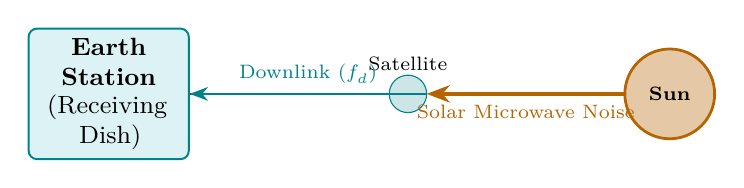
\begin{tikzpicture}[scale=0.95, every node/.style={font=\scriptsize}]
  % Sun (Right side)
  \fill[color=myamber!35, draw=myamber, line width=1pt] (5,0) circle (0.6cm);
  \node at (5,0) {\textbf{Sun}};
  
  % Satellite (Center)
  \fill[color=myteal!20, draw=myteal] (1.5,0) circle (0.25cm);
  \node at (1.5,0.4) {Satellite};
  
  % Earth Station (Left side)
  \node[block, text width=1.8cm] (es) at (-2.5,0) {\textbf{Earth Station}\\[-1pt](Receiving Dish)};
  
  % Alignment line
  \draw[color=myred, thick, dashed] (es.east) -- (1.25,0);
  \draw[arrow, color=myteal] (1.75,0) -- node[midway, above] {Downlink ($f_d$)} (es.east);
  \draw[arrow, color=myamber, line width=1.2pt] (4.4,0) -- node[midway, below, color=myamber] {Solar Microwave Noise} (1.75,0);
\end{tikzpicture}
\end{tcolorbox}

\begin{itemize}[leftmargin=*, itemsep=4pt]
  \item \textbf{Effects:} The Sun acts as an extremely high-temperature noise source ($T_{sun} > 10,000 \text{ K}$ at microwave frequencies). The antenna noise temperature ($T_{ant}$) spikes, reducing the receiver's carrier-to-noise ratio ($C/N$) to near zero, resulting in a complete communications dropout lasting up to 10 minutes.
  \item \textbf{Remedies:} Sun outages cannot be prevented physically. Ground operators mitigate the impact by:
    \begin{itemize}[leftmargin=*, itemsep=2pt, topsep=2pt]
      \item Rerouting critical traffic to adjacent satellites.
      \item Using dual-antenna setups pointed at different orbital slots.
    \end{itemize}
\end{itemize}

% ===============================================================================
\section{Doppler Frequency Shift}
% ===============================================================================

When a satellite moves relative to a terrestrial Earth station, the received frequency shifts from the transmitted frequency due to the Doppler effect.

\begin{tcolorbox}[defbox]
\textbf{Doppler Shift:} The change in apparent frequency of a received electromagnetic wave caused by relative motion between the transmitter (satellite) and receiver (ground station).
\end{tcolorbox}

\subsection{Mathematical Expression for Doppler Shift}
Let a satellite move with velocity vector $\mathbf{v}$ making an angle $\theta$ relative to the line of sight (LOS) to the Earth station.

\begin{tcolorbox}[tikzbox, title={Doppler Vector Components}]
\centering
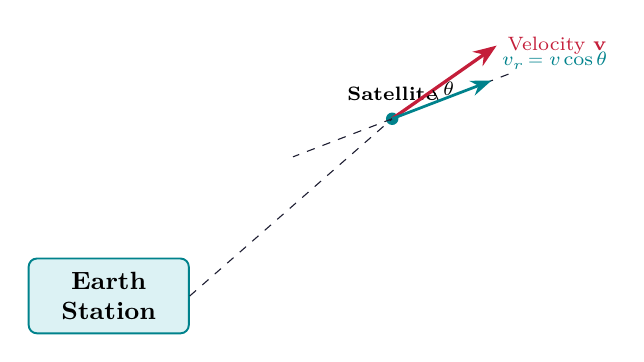
\begin{tikzpicture}[scale=0.9, every node/.style={font=\scriptsize}]
  % Earth Station
  \node[block, text width=1.8cm] (es) at (0,0) {\textbf{Earth Station}};
  
  % Satellite
  \coordinate (Sat) at (4,2.5);
  \fill[color=myteal] (Sat) circle (2.5pt);
  \node[above=0.1cm of Sat] {\textbf{Satellite}};
  
  % Velocity Vector
  \draw[arrow, color=myred, line width=1.2pt] (Sat) -- ($(Sat)+(35:1.8)$) node[right, color=myred] {Velocity $\mathbf{v}$};
  
  % Line of Sight (LOS)
  \draw[dashed, color=mydark] (es.east) -- (Sat);
  
  % Extended LOS from satellite
  \draw[dashed, color=mydark] (Sat) -- ($(Sat)+(201:1.5)$);
  \draw[dashed, color=mydark] (Sat) -- ($(Sat)+(21:1.8)$) coordinate (los_ext);
  
  % Angle theta
  \draw (Sat) +(21:0.7cm) arc (21:35:0.7cm);
  \node at ($(Sat)+(28:0.9cm)$) {$\theta$};
  
  % Projection (radial velocity)
  \draw[arrow, color=myteal, line width=1pt] (Sat) -- ($(Sat)+(21:1.5)$) node[above right, color=myteal] {$v_r = v\cos\theta$};
\end{tikzpicture}
\end{tcolorbox}

The relative radial velocity ($v_r$) along the line of sight is:
\begin{equation}
  v_r = v \cos(\theta)
\end{equation}
If $f$ is the transmitted frequency and $c$ is the speed of light, the received frequency $f'$ is:
\begin{equation}
  f' = f \left( 1 \pm \frac{v_r}{c} \right)
\end{equation}
The Doppler frequency shift ($\Delta f$) is defined as:
\begin{equation}
  \Delta f = f' - f = \pm f \frac{v_r}{c} = \pm \frac{v \cos(\theta)}{\lambda}
\end{equation}

Where:
\begin{itemize}[leftmargin=*, itemsep=3pt]
  \item $\Delta f$ = Doppler frequency shift (Hz)
  \item $f$ = Transmitted carrier frequency (Hz)
  \item $v_r = v \cos(\theta)$ = Radial velocity component (m/s)
  \item $c \approx 3 \times 10^8$ m/s = Speed of light
  \item The sign is \textbf{positive (+)} when the satellite is approaching the station.
  \item The sign is \textbf{negative (-)} when the satellite is receding from the station.
\end{itemize}

\subsection{Impact on Satcom Systems}
\begin{enumerate}[label=\textbf{\arabic*.}, leftmargin=*, itemsep=3pt]
  \item \textbf{High Frequency Vulnerability:} Since $\Delta f \propto f$, Doppler shift is severe at high frequencies (Ku and Ka bands) and in Low Earth Orbit (LEO) systems where orbital speed is extremely high ($v \approx 7.5$ km/s).
  \item \textbf{Receiver Tracking:} Receiver circuits must implement automatic frequency control (AFC) loops to track the frequency drift and maintain demodulator lock.
\end{enumerate}

% ===============================================================================
% MANDATORY QUICK REVISION PAGE
% ===============================================================================
\newpage
\begin{center}
  {\large\bfseries\color{myred} Quick Revision --- Module IV}\\[3pt]
  {\small\color{mydark} Typical Phenomena in Satellite Communication $|$ PE-EC701B}
\end{center}
\noindent{\color{myred}\rule{\linewidth}{1.2pt}}
\vspace{4pt}

\begin{tcolorbox}[formulabox, title={\textbf{Key Formulas at a Glance}}]
\renewcommand{\arraystretch}{1.9}
\begin{tabularx}{\linewidth}{B{5.0cm} X}Doppler Frequency Shift & $\displaystyle \Delta f = \pm f \frac{v_r}{c} = \pm \frac{v_r}{\lambda}$ \\[4pt]
Relative Radial Velocity & $v_r = v \cos(\theta)$ \\[4pt]
Maximum Eclipse Duration & $t_{max} \approx 72 \text{ minutes}$ (occurs at Equinox center) \\[4pt]
Doppler Shift (Approaching) & $\displaystyle f_{received} = f_{transmitted} \left( 1 + \frac{v_r}{c} \right)$
\end{tabularx}
\end{tcolorbox}

\begin{tcolorbox}[defbox, title={\textbf{One-Line Definitions}}]
\begin{itemize}[leftmargin=*, itemsep=2.5pt, topsep=0pt]
  \item \textbf{Solar Eclipse:} Temporary blockage of sunlight to a satellite by Earth's shadow.
  \item \textbf{Equinox:} The twice-yearly period (March/September) when solar eclipses occur for GEO satellites.
  \item \textbf{Sun Transit Outage:} Alignment of ground station, satellite, and Sun, causing thermal noise outages.
  \item \textbf{Doppler Shift:} Apparent frequency deviation of a carrier wave due to relative motion.
  \item \textbf{Radial Velocity ($v_r$):} The component of satellite velocity directly along the ground station line of sight.
  \item \textbf{Umbra:} The central, completely dark portion of Earth's shadow.
  \item \textbf{AFC:} Automatic Frequency Control, used to dynamically track Doppler carrier shifts.
\end{itemize}
\end{tcolorbox}

\begin{tcolorbox}[exambox, title={\textbf{Frequently Asked / Viva Questions}}]
\begin{enumerate}[topsep=0pt, label=\textbf{Q\arabic*.}, itemsep=5pt]
  \item \Q{Why do GEO satellites experience eclipses only during equinoxes?}
    Because the Earth's orbital plane is tilted at $23.4^\circ$. Eclipses occur only when the Sun crosses the equator (during spring and autumn equinoxes), aligning the Sun, Earth, and satellite.
  \item \Q{What are the major effects of a solar eclipse on a satellite?}
    Complete loss of primary solar power generation (requiring battery operation) and severe thermal shock (temperatures drop from $+100^\circ\text{C}$ to $-100^\circ\text{C}$).
  \item \Q{How does a satellite thermal control system mitigate eclipse effects?}
    It activates electric heaters to maintain minimum operating temperatures for sensitive electronics and uses multi-layer insulation (MLI) to retain heat.
  \item \Q{Explain the physical cause of a Sun Transit Outage.}
    The Sun is a massive blackbody radiator emitting intense microwave noise. When aligned behind the satellite, this thermal noise fills the ground receiver dish beam, blocking the satellite downlink.
  \item \Q{State the duration and annual schedule of Sun Transit Outages.}
    They occur twice a year (near equinoxes) for a few consecutive days, lasting about 2 to 10 minutes per day.
  \item \Q{Derive the mathematical expression for Doppler frequency shift.}
    Let a source emit waves of period $T$. Due to radial motion $v_r$, the wave travels distance $v_r T$ per cycle. The change in apparent wavelength is $\Delta \lambda = \pm v_r / f$. Since $f = c/\lambda$, differentiating yields $\Delta f = \pm f(v_r/c)$.
  \item \Q{Under what conditions is Doppler shift maximum and zero?}
    Doppler shift is maximum when $\theta = 0^\circ$ (satellite is moving directly toward or away from the station). It is zero when $\theta = 90^\circ$ (satellite motion is perpendicular to the line of sight).
  \item \Q{Why is Doppler shift more severe in LEO satellites than in GEO satellites?}
    LEO satellites travel at extremely high speeds (~7.5 km/s) relative to Earth, creating huge radial velocity changes. GEO satellites are relatively stationary, experiencing negligible Doppler shift.
  \item \Q{Calculate the maximum Doppler shift for a LEO satellite ($v_r = 7 \text{ km/s}$) transmitting at 10 GHz.}
    $\Delta f = f \cdot (v_r/c) = 10^{10} \times (7 \times 10^3) / (3 \times 10^8) = 7 \times 10^{13} / (3 \times 10^8) \approx 233.33 \text{ kHz}$.
  \item \Q{What is the difference between Umbra and Penumbra?}
    Umbra is the inner region of the shadow where the light source is completely blocked. Penumbra is the outer region where only a portion of the light source is blocked.
  \item \Q{Why are Sun outages independent of the satellite's power status?}
    Because they are caused by external solar noise interfering with the ground receiver, not by any power loss on the satellite itself.
  \item \Q{How does a ground receiver maintain lock during a high Doppler LEO pass?}
    By using a phase-locked loop (PLL) with wide tracking bandwidth or digital frequency estimation algorithms to dynamically adjust the receiver local oscillator.
\end{enumerate}
\end{tcolorbox}

\begin{tcolorbox}[tikzbox, title={Comparison of Solar Eclipse and Sun Transit Outage}]
\renewcommand{\arraystretch}{1.4}
\par\noindent
{\renewcommand{\arraystretch}{1.55}%
\begin{tabularx}{\linewidth}{|B{3.2cm}|Y|Y|}\hline
\textbf{Parameter} & \textbf{\color{myteal}Solar Eclipse} & \textbf{\color{myamber}Sun Transit Outage} \\[4pt]
\hline
\textbf{Affected Unit} & Satellite (Spacecraft) & Ground Station (Earth Terminal) \\
\hline
\textbf{Physical Cause} & Earth blocks solar light to the satellite. & Sun aligns behind the satellite. \\[4pt]
\hline
\textbf{Primary Effect} & Loss of solar power, temperature drop. & Severe thermal noise, downlink carrier loss. \\[4pt]
\hline
\textbf{System Remedy} & Secondary batteries, thermal heaters. & Traffic rerouting, antenna diversity. \\[4pt]
\hline
\textbf{Max Duration} & Up to 72 minutes per day. & Up to 10 minutes per day. \\
\hline
\end{tabularx}
}
\end{tcolorbox}


% -- Module 5 -----------------------------------------------------------------
\modulestart{5}{Power Flux Density and Received Signal Power}

\section{Power Flux Density and Received Signal Power}
% ===============================================================================

The link budget calculations track the signal power level from the ground transmitter, through the orbital space path, to the ground receiver.

\subsection{Power Flux Density (F)}
An isotropic radiator distributes its power uniformly in all directions over a sphere. At a distance $d$ from the transmitter, the power flux density ($F$) is:
\begin{equation}
  F = \frac{P_t}{4\pi d^2} \quad [\text{W/m}^2]
\end{equation}
If the transmitter uses a directional antenna with gain $G_t$, the power is concentrated, yielding:
\begin{equation}
  F = \frac{P_t G_t}{4\pi d^2} = \frac{EIRP}{4\pi d^2} \quad [\text{W/m}^2]
\end{equation}
Where $EIRP = P_t G_t$ is the \textbf{Equivalent Isotropically Radiated Power}.

\subsection{Received Signal Power ($P_r$)}
The receiving antenna intercepts a portion of this flux. The captured power is proportional to the antenna's \textbf{effective aperture area} ($A_e$):
\begin{equation}
  P_r = F \cdot A_e \quad [\text{W}]
\end{equation}
Using the fundamental antenna relation $A_e = \frac{G_r \lambda^2}{4\pi}$:
\begin{equation}
  P_r = \left( \frac{P_t G_t}{4\pi d^2} \right) \left( \frac{G_r \lambda^2}{4\pi} \right) = P_t G_t G_r \left( \frac{\lambda}{4\pi d} \right)^2 \quad [\text{W}]
\end{equation}
This is the \textbf{Friis Transmission Equation}. It can be written as:
\begin{equation}
  P_r = \frac{EIRP \cdot G_r}{L_{FSL}}
\end{equation}
Where $L_{FSL}$ is the \textbf{Free Space Path Loss (FSL)}:
\begin{equation}
  L_{FSL} = \left( \frac{4\pi d}{\lambda} \right)^2 = \left( \frac{4\pi f d}{c} \right)^2
\end{equation}
In decibels:
\begin{equation}
  L_{FSL\_dB} = 32.44 + 20\log_{10}(d_{\text{km}}) + 20\log_{10}(f_{\text{MHz}})
\end{equation}

% ===============================================================================
\section{System Noise Temperature and Noise Power}
% ===============================================================================

The performance of a receiving system is limited by thermal noise, which is modeled using an equivalent noise temperature.

\subsection{Noise Power Calculation}
The thermal noise power ($N$) generated in a receiver of bandwidth $B$ is given by:
\begin{equation}
  N = k \cdot T_s \cdot B \quad [\text{W}]
\end{equation}
Where:
\begin{itemize}[leftmargin=*, itemsep=3pt]
  \item $k = 1.38 \times 10^{-23} \text{ J/K}$ (Boltzmann's constant)
  \item $T_s$ = System Noise Temperature (Kelvin, K)
  \item $B$ = Noise Bandwidth (Hz)
\end{itemize}
In dBW:
\begin{equation}
  N_{\text{dBW}} = -228.6 + 10\log_{10}(T_s) + 10\log_{10}(B)
\end{equation}

\subsection{Calculation of System Noise Temperature ($T_s$)}
If an antenna with noise temperature $T_{ant}$ is connected to a receiver via a lossy waveguide line with loss factor $L$ ($L \ge 1$, where $L = 10^{\text{Loss\_dB}/10}$) at physical temperature $T_0 \approx 290\text{ K}$, the system noise temperature ($T_s$) referred to the receiver input is:
\begin{equation}
  T_s = \frac{T_{ant}}{L} + T_{0}\left(1 - \frac{1}{L}\right) + T_{rx}
\end{equation}
Where $T_{rx}$ is the effective noise temperature of the receiver itself, related to its noise figure $F_{rx}$ by:
\begin{equation}
  T_{rx} = T_0 (F_{rx} - 1)
\end{equation}

For a cascaded chain of amplifiers (e.g., LNA followed by mixer and down-converter), the overall receiver noise temperature is given by \textbf{Friis Formula}:
\begin{equation}
  T_{rx} = T_1 + \frac{T_2}{G_1} + \frac{T_3}{G_1 G_2} + \dots
\end{equation}
Where $T_n$ and $G_n$ are the equivalent noise temperature and linear gain of the $n$-th stage. This formula proves why a high-gain, low-noise LNA must be the first stage.

% ===============================================================================
\section{Drafting the Satellite Link Budget}
% ===============================================================================

The link budget is a tabular summation of all gains and losses along the communication path to calculate the final \textbf{Carrier-to-Noise Ratio ($C/N$)} at the receiver demodulator.

\begin{tcolorbox}[tikzbox, title={Link Budget System Model}]
\centering
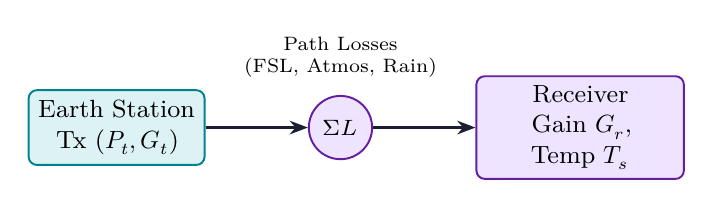
\begin{tikzpicture}[scale=0.9, every node/.style={font=\scriptsize}]
  % Ground Station
  \node[block, text width=2.0cm] (tx) {Earth Station\\Tx ($P_t, G_t$)};
  
  % Path
  \node[snode, right=1.3cm of tx] (loss) {$\Sigma L$};
  \node[above=0.1cm of loss, align=center] {Path Losses\\(FSL, Atmos, Rain)};
  
  % Satellite Receiver
  \node[block, right=1.3cm of loss, draw=mypurple, fill=hdrpurple] (sat) {Receiver\\Gain $G_r$, Temp $T_s$};
  
  % Connections
  \draw[arrow] (tx) -- (loss);
  \draw[arrow] (loss) -- (sat);
\end{tikzpicture}
\end{tcolorbox}

\subsection{Carrier-to-Noise Ratio (C/N) Expression}
The received carrier power is $C = P_r$. The carrier-to-noise ratio is:
\begin{equation}
  \frac{C}{N} = \frac{P_r}{k T_s B} = \frac{EIRP \cdot G_r}{L_{\text{losses}} \cdot k T_s B} = \left(\frac{EIRP}{L_{\text{losses}} \cdot k \cdot B}\right) \left(\frac{G_r}{T_s}\right)
\end{equation}
Where $G/T = G_r/T_s$ is the receiving system's \textbf{Figure of Merit} (expressed in $\text{dB/K}$).

In logarithmic decibel form:
\begin{equation}
  \left[\frac{C}{N}\right]_{\text{dB}} = EIRP_{\text{dBW}} - L_{\text{losses\_dB}} + \left[\frac{G}{T}\right]_{\text{dB/K}} - k_{\text{dBW}} - B_{\text{dB-Hz}}
\end{equation}
Where:
\begin{itemize}[leftmargin=*, itemsep=3pt]
  \item $k_{\text{dBW}} = -228.6 \text{ dBW/(K}\cdot\text{Hz)}$
  \item $B_{\text{dB-Hz}} = 10\log_{10}(B_{\text{Hz}})$
  \item $L_{\text{losses\_dB}} = L_{FSL} + L_{\text{atmospheric}} + L_{\text{polarization}} + L_{\text{antenna-pointing}}$
\end{itemize}

\subsection{Carrier-to-Noise Density Ratio ($C/N_0$)}
To evaluate system performance independent of receiver bandwidth, we use $C/N_0$:
\begin{equation}
  \frac{C}{N_0} = \frac{C}{N} \cdot B \quad [\text{Hz}]
\end{equation}
\begin{equation}
  \left[\frac{C}{N_0}\right]_{\text{dB-Hz}} = EIRP_{\text{dBW}} - L_{\text{losses\_dB}} + \left[\frac{G}{T}\right]_{\text{dB/K}} + 228.6
\end{equation}

% ===============================================================================
\section{Link Performance: Clear Air vs. Rainy Conditions}
% ===============================================================================

Atmospheric phenomena significantly degrade link performance, especially at frequencies above 10 GHz (Ku and Ka bands).

\subsection{Clear Air Conditions}
Under clear skies, the link is subject only to \textbf{gaseous absorption} from water vapor and oxygen molecules in the atmosphere. The attenuation is low (typically $< 0.5$ dB for C-band).

\subsection{Rainy Conditions}
Rain introduces a dual penalty on the link:
\begin{enumerate}[label=\textbf{\arabic*.}, leftmargin=*, itemsep=3pt]
  \item \textbf{Signal Attenuation ($A_{\text{rain}}$):} Rain droplets scatter and absorb the microwave energy, reducing the received carrier power ($C$) by $A_{\text{rain}}$ dB.
  \item \textbf{Increase in Noise Temperature ($\Delta T_{\text{ant}}$):} The absorbing rain medium acts as a thermal radiator, increasing the antenna noise temperature:
    \begin{equation}
      T_{ant\_rain} = T_{ant\_clear} \cdot 10^{-A_{\text{rain}}/10} + T_m \left( 1 - 10^{-A_{\text{rain}}/10} \right)
    \end{equation}
    Where $T_m$ is the physical temperature of the rain medium (typically assumed to be $275\text{ K}$ or $290\text{ K}$).
\end{enumerate}

This increase in $T_{ant}$ directly raises the system noise temperature $T_s$, thereby raising the noise floor ($N$). This combined effect severely degrades the overall received $[C/N]$ ratio.

% ===============================================================================
% MANDATORY QUICK REVISION PAGE
% ===============================================================================
\newpage
\begin{center}
  {\large\bfseries\color{myred} Quick Revision --- Module V}\\[3pt]
  {\small\color{mydark} Satellite Link Budget $|$ PE-EC701B}
\end{center}
\noindent{\color{myred}\rule{\linewidth}{1.2pt}}
\vspace{4pt}

\begin{tcolorbox}[formulabox, title={\textbf{Key Formulas at a Glance}}]
\renewcommand{\arraystretch}{1.9}
\begin{tabularx}{\linewidth}{B{5.0cm} X}Equivalent Radiated Power & $EIRP = P_t G_t \implies EIRP_{\text{dBW}} = P_{t\text{\,dBW}} + G_{t\text{\,dBi}}$ \\[4pt]
Free Space Path Loss & $\displaystyle L_{FSL} = \left(\frac{4\pi d}{\lambda}\right)^2 \implies L_{FSL\_dB} \approx 32.44 + 20\log(d_{\text{km}}) + 20\log(f_{\text{MHz}})$ \\[4pt]
Noise Power & $N = k T_s B \implies N_{\text{dBW}} = -228.6 + 10\log(T_s) + 10\log(B)$ \\[4pt]
Friis Cascade Temperature & $\displaystyle T_{rx} = T_1 + \frac{T_2}{G_1} + \frac{T_3}{G_1 G_2} + \dots$ \\[4pt]
Carrier-to-Noise Ratio & $\displaystyle \left[\frac{C}{N}\right]_{\text{dB}} = EIRP_{\text{dBW}} - L_{\text{losses\_dB}} + \left[\frac{G}{T}\right]_{\text{dB/K}} - 10\log(B) + 228.6$
\end{tabularx}
\end{tcolorbox}

\begin{tcolorbox}[defbox, title={\textbf{One-Line Definitions}}]
\begin{itemize}[leftmargin=*, itemsep=2.5pt, topsep=0pt]
  \item \textbf{EIRP:} Equivalent power that would need to be radiated by an isotropic antenna to achieve the same directional signal strength.
  \item \textbf{Free Space Loss:} Geometrical spreading loss of electromagnetic energy as it radiates outward through space.
  \item \textbf{G/T Ratio:} Figure of merit of a receiving system, representing the ratio of antenna gain to system noise temperature.
  \item \textbf{Friis Formula:} Expression calculating the total noise temperature of cascaded receiver stages.
  \item \textbf{Boltzmann's Constant (k):} Proportionality constant relating kinetic energy to temperature ($1.38 \times 10^{-23} \text{ J/K}$).
  \item \textbf{Rain Fade Penalty:} Combined loss of carrier power and rise in receiver noise floor caused by rain.
\end{itemize}
\end{tcolorbox}

\begin{tcolorbox}[exambox, title={\textbf{Frequently Asked / Viva Questions}}]
\begin{enumerate}[topsep=0pt, label=\textbf{Q\arabic*.}, itemsep=5pt]
  \item \Q{Define EIRP and write its equation in logarithmic form.}
    Equivalent Isotropically Radiated Power. It measures the total directional power radiated. $EIRP_{\text{dBW}} = P_{t\text{\,dBW}} + G_{t\text{\,dBi}}$.
  \item \Q{What is Free Space Path Loss (FSL) and why does it occur?}
    It is the attenuation of a wave due to the spherical spreading of its energy over distance. $L_{FSL} = (4\pi d/\lambda)^2$. It does not represent energy absorption by matter.
  \item \Q{Explain the physical meaning of the G/T ratio.}
    It is the receiver's Figure of Merit. A higher $G/T$ indicates a highly sensitive receiving station (high gain $G$ or low system noise temperature $T$).
  \item \Q{How does the first stage of a receiver cascade affect its noise performance?}
    According to Friis Formula ($T_{rx} = T_1 + T_2/G_1 + \dots$), if the first stage has high gain ($G_1$), it divides and minimizes the noise contributions of all subsequent stages ($T_2, T_3$). Thus, the first stage dictates the overall noise figure.
  \item \Q{Calculate the noise power (in dBW) for a 36 MHz transponder bandwidth at a system temperature of 400 K.}
    $N = -228.6 + 10\log(400) + 10\log(36 \times 10^6) = -228.6 + 26.02 + 75.56 = -127.02 \text{ dBW}$.
  \item \Q{What is the difference between $C/N$ and $C/N_0$?}
    $C/N$ is the carrier-to-noise ratio within a specific bandwidth $B$. $C/N_0$ is the carrier-to-noise density ratio, normalized to a 1 Hz bandwidth ($C/N_0 = (C/N) \cdot B$).
  \item \Q{Explain the dual penalty rain inflicts on satellite links.}
    Rain absorbs and scatters the carrier signal, reducing $C$. Simultaneously, the absorbing rain emits thermal noise, increasing the antenna temperature and raising the noise floor $N$.
  \item \Q{An Earth station has a dish antenna with 40 dBi gain and an LNA with 100 K noise temperature. The antenna noise temperature is 50 K under clear skies. Calculate the clear-sky G/T.}
    $T_s = T_{ant} + T_{rx} = 50 + 100 = 150 \text{ K}$. $G/T = 40 - 10\log_{10}(150) = 40 - 21.76 = 18.24 \text{ dB/K}$.
  \item \Q{What is the physical temperature $T_0$ used in noise figure definitions and what is its value?}
    It is the standard reference temperature for noise measurements, defined as $290\text{ K}$ ($17^\circ\text{C}$).
  \item \Q{Why are link margins drafted into satellite designs?}
    A link margin (typically 3 to 6 dB) is added to ensure the system remains operational during atmospheric degradation, rain fade, or antenna pointing errors.
  \item \Q{Write the relation between Noise Figure ($F$) and equivalent noise temperature ($T_e$).}
    $T_e = T_0(F - 1)$ where $T_0 = 290\text{ K}$.
  \item \Q{How does the slant path impact rain attenuation in satellite links?}
    A lower elevation angle increases the slant path length through the rain cell, which increases the total rain attenuation compared to a vertical path.
\end{enumerate}
\tcbset{colbacktitle=myteal, coltitle=white}
\end{tcolorbox}

\begin{tcolorbox}[tikzbox, title={Drafting a Sample Link Budget Table}]
\renewcommand{\arraystretch}{1.4}
\par\noindent
{\renewcommand{\arraystretch}{1.65}%
\begin{tabularx}{\linewidth}{|B{3.5cm}|Y|Y|}\hline
\textbf{Link Parameter} & \textbf{Value (Clear Air)} & \textbf{Value (Rainy - 3 dB fade)} \\
\hline
Transmitter Power ($P_t$) & $10 \text{ dBW}$ & $10 \text{ dBW}$ \\[4pt]
\hline
Transmit Antenna Gain ($G_t$) & $45 \text{ dBi}$ & $45 \text{ dBi}$ \\[4pt]
\hline
\textbf{EIRP} & $\mathbf{55 \text{ dBW}}$ & $\mathbf{55 \text{ dBW}}$ \\[4pt]
\hline
Free Space Loss ($L_{FSL}$) & $-200 \text{ dB}$ & $-200 \text{ dB}$ \\[4pt]
\hline
Atmospheric/Rain Loss ($L_a$) & $-0.5 \text{ dB}$ & $-3.5 \text{ dB}$ (includes rain) \\[4pt]
\hline
Receiver Antenna Gain ($G_r$) & $35 \text{ dBi}$ & $35 \text{ dBi}$ \\[4pt]
\hline
System Noise Temp ($T_s$) & $150 \text{ K}$ ($21.8 \text{ dB-K}$) & $250 \text{ K}$ ($24.0 \text{ dB-K}$) (increases due to rain) \\[4pt]
\hline
Boltzmann Constant ($k$) & $-228.6 \text{ dBW/Hz-K}$ & $-228.6 \text{ dBW/Hz-K}$ \\
\hline
\textbf{C/N$_0$ Ratio} & $\mathbf{96.3 \text{ dB-Hz}}$ & $\mathbf{91.1 \text{ dB-Hz}}$ \\[4pt]
\hline
\end{tabularx}
}
\end{tcolorbox}


% -- Module 6 -----------------------------------------------------------------
\modulestart{6}{Modulation Schemes in Satellite Communication}

\section{Modulation Schemes in Satellite Communication}
% ===============================================================================

Modulation is the process of mapping digital baseband information onto a high-frequency analog carrier wave suitable for transmission through space.

\begin{tcolorbox}[defbox]
\textbf{Digital Modulation in Satcom:} The translation of binary sequences into discrete phase or amplitude shifts of a microwave carrier. Because satellite transponders are power-limited, phase-shift keying (PSK) schemes like QPSK are preferred over amplitude-modulated schemes.
\end{tcolorbox}

\subsection{Why QPSK is the Industry Workhorse}
\begin{itemize}[leftmargin=*, itemsep=3.5pt]
  \item \textbf{Constant Envelope:} QPSK has a constant envelope (its amplitude does not vary with phase shifts). This allows the satellite high-power amplifier (HPA) to operate at its maximum efficiency point (saturation) without introducing severe \textbf{amplitude-to-phase distortion (AM/PM)}.
  \item \textbf{Spectral Efficiency:} QPSK offers double the spectral efficiency of BPSK ($2 \text{ bps/Hz}$ vs. $1 \text{ bps/Hz}$) for the same noise performance.
  \item \textbf{Higher-Order Modulation:} Systems requiring higher data rates (such as DTH satellite TV) use \textbf{8PSK} or \textbf{16APSK} (Amplitude Phase Shift Keying) coupled with advanced forward error correction (FEC) under the DVB-S2 standard.
\end{itemize}

% ===============================================================================
\section{Concept of Multiple Access}
% ===============================================================================

A communication satellite serves as a central hub. \textbf{Multiple Access} is the set of traffic-sharing protocols that allow multiple geographically separated ground terminals to transmit signals simultaneously through a single satellite transponder.

\begin{tcolorbox}[defbox]
\textbf{Multiple Access:} The technique of sharing a common channel resource (transponder bandwidth and power) among multiple users without causing mutual electromagnetic interference.
\end{tcolorbox}

\subsection{Sharing Methodologies}
The three primary sharing mechanisms are:
\begin{enumerate}[label=\textbf{\arabic*.}, leftmargin=*, itemsep=2.5pt]
  \item \textbf{FDMA:} Resource split by Frequency.
  \item \textbf{TDMA:} Resource split by Time.
  \item \textbf{CDMA:} Resource split by mathematical Codes.
\end{enumerate}

\begin{tcolorbox}[tikzbox, title={Multiple Access Resource Partitioning}]
\centering
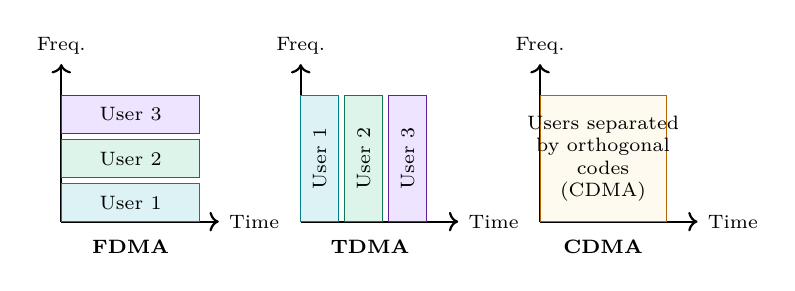
\begin{tikzpicture}[scale=0.8, every node/.style={font=\scriptsize}]
  % FDMA Grid
  \begin{scope}[xshift=0cm]
    \draw[thick, ->] (0,0) -- (2.5,0) node[right] {Time};
    \draw[thick, ->] (0,0) -- (0,2.5) node[above] {Freq.};
    \draw[fill=hdrteal, draw=myteal] (0,0) rectangle (2.2,0.6);
    \draw[fill=hdrgreen, draw=mygreen] (0,0.7) rectangle (2.2,1.3);
    \draw[fill=hdrpurple, draw=mypurple] (0,1.4) rectangle (2.2,2.0);
    \node at (1.1,0.3) {User 1};
    \node at (1.1,1.0) {User 2};
    \node at (1.1,1.7) {User 3};
    \node at (1.1,-0.4) {\textbf{FDMA}};
  \end{scope}
  
  % TDMA Grid
  \begin{scope}[xshift=3.8cm]
    \draw[thick, ->] (0,0) -- (2.5,0) node[right] {Time};
    \draw[thick, ->] (0,0) -- (0,2.5) node[above] {Freq.};
    \draw[fill=hdrteal, draw=myteal] (0,0) rectangle (0.6,2.0);
    \draw[fill=hdrgreen, draw=mygreen] (0.7,0) rectangle (1.3,2.0);
    \draw[fill=hdrpurple, draw=mypurple] (1.4,0) rectangle (2.0,2.0);
    \node[rotate=90] at (0.3,1.0) {User 1};
    \node[rotate=90] at (1.0,1.0) {User 2};
    \node[rotate=90] at (1.7,1.0) {User 3};
    \node at (1.1,-0.4) {\textbf{TDMA}};
  \end{scope}
  
  % CDMA Grid
  \begin{scope}[xshift=7.6cm]
    \draw[thick, ->] (0,0) -- (2.5,0) node[right] {Time};
    \draw[thick, ->] (0,0) -- (0,2.5) node[above] {Freq.};
    \draw[fill=hdramber!40, draw=myamber] (0,0) rectangle (2.0,2.0);
    \node[align=center] at (1.0,1.0) {Users separated\\by orthogonal\\codes\\(CDMA)};
    \node at (1.0,-0.4) {\textbf{CDMA}};
  \end{scope}
\end{tikzpicture}
\tcbset{colbacktitle=myteal, coltitle=white}
\end{tcolorbox}

% ===============================================================================
\section{Frequency Division Multiple Access (FDMA)}
% ===============================================================================

In FDMA, the transponder bandwidth is divided into smaller, non-overlapping frequency channels. Each Earth station is assigned a dedicated carrier frequency and transmits continuously.

\subsection{FDM vs. FDMA}
\begin{itemize}[leftmargin=*, itemsep=3.5pt]
  \item \textbf{FDM (Frequency Division Multiplexing):} A terrestrial process where multiple analog signals are combined at a single transmitter into a single composite signal.
  \item \textbf{FDMA (Multiple Access):} An uplink sharing process where multiple physically separate ground transmitters send distinct carriers to the satellite.
\end{itemize}

\subsection{Intermodulation Noise and Back-Off}
When multiple carrier waves pass through the satellite's high-power amplifier (HPA), the HPA's non-linear characteristics mix the carriers, generating \textbf{intermodulation distortion (IMD)} products.
To minimize IMD, the amplifier must be operated in its linear region rather than at saturation. This requires \textbf{Amplifier Back-Off}:
\begin{itemize}[leftmargin=*, itemsep=3.5pt]
  \item \textbf{Input Back-Off (IBO):} Reducing the input signal power below the level that drives the HPA to saturation.
  \item \textbf{Output Back-Off (OBO):} The resulting reduction in output transmit power (typically 3 to 6 dB), which reduces transponder efficiency.
\end{itemize}

% ===============================================================================
\section{Time Division Multiple Access (TDMA)}
% ===============================================================================

In TDMA, the entire transponder bandwidth is allocated to one Earth station at a time. Each station transmits data in high-speed, non-overlapping periodic bursts.

\subsection{TDMA Frame Structure}
The transmissions are organized into periodic TDMA frames. A frame consists of a preamble and traffic bursts.

\begin{itemize}[leftmargin=*, itemsep=3.5pt]
  \item \textbf{Preamble:} Contains carrier synchronization bits and unique words for time alignment.
  \item \textbf{Guard Times ($t_g$):} Small silent intervals left between adjacent bursts to prevent overlap caused by propagation delay variations.
\end{itemize}

\subsection{Frame Efficiency (\texorpdfstring{$\eta_f$}{eta\_f})}
Because guard times and preambles carry no user information, they represent overhead. The frame efficiency ($\eta_f$) is:
\begin{equation}
  \eta_f = 1 - \frac{T_{overhead}}{T_f} = 1 - \frac{N \cdot t_{preamble} + N \cdot t_g}{T_f}
\end{equation}
Where:
\begin{itemize}[leftmargin=*, itemsep=3pt]
  \item $T_f$ = Total frame duration
  \item $N$ = Number of traffic bursts (users) in the frame
  \item $t_{preamble}$ = Duration of the preamble sequence
  \item $t_g$ = Guard time duration
\end{itemize}

% ===============================================================================
\section{Code Division Multiple Access (CDMA)}
% ===============================================================================

In CDMA, all Earth stations transmit simultaneously over the entire transponder bandwidth. Users are separated using unique, orthogonal pseudo-noise (PN) codes.

\subsection{Direct Sequence Spread Spectrum (DS-CDMA)}
The baseband binary data stream is multiplied by a high-rate PN code (chipping sequence). This spreads the signal bandwidth over the entire transponder band. At the receiver, the signal is multiplied by the identical synchronized PN code to collapse the signal back to its original bandwidth (de-spreading), while all other users' signals remain spread as low-power background noise.

\subsection{Processing Gain ($G_p$)}
The ratio of the spread bandwidth ($B_{ss}$) to the baseband data bandwidth ($B_{data}$) determines the processing gain:
\begin{equation}
  G_p = \frac{B_{ss}}{B_{data}} \approx \frac{R_c}{R_d}
\end{equation}
Where $R_c$ is the chip rate (chips/sec) and $R_d$ is the baseband data rate (bits/sec).
In decibels:
\begin{equation}
  G_{p\_dB} = 10 \log_{10}\left( \frac{R_c}{R_d} \right)
\end{equation}
A higher processing gain provides greater immunity to interference and jamming.

% ===============================================================================
% MANDATORY QUICK REVISION PAGE
% ===============================================================================
\newpage
\begin{center}
  {\large\bfseries\color{myred} Quick Revision --- Module VI}\\[3pt]
  {\small\color{mydark} Modulation and Multiple Access Schemes $|$ PE-EC701B}
\end{center}
\noindent{\color{myred}\rule{\linewidth}{1.2pt}}
\vspace{4pt}

\begin{tcolorbox}[formulabox, title={\textbf{Key Formulas at a Glance}}]
\renewcommand{\arraystretch}{1.9}
\begin{tabularx}{\linewidth}{B{5.0cm} X}QPSK Bandwidth Efficiency & $\displaystyle \eta_{bps} = \frac{R}{B} = 2 \text{ bits/sec/Hz}$ \\[4pt]
TDMA Frame Efficiency & $\displaystyle \eta_f = 1 - \frac{N(t_{preamble} + t_g)}{T_f}$ \\[4pt]
CDMA Processing Gain & $\displaystyle G_p = \frac{B_{ss}}{B_{data}} \approx \frac{R_c}{R_d}$ \\[4pt]
IMD Product Frequencies & $f_{IMD} = 2f_1 - f_2$ \quad and \quad $2f_2 - f_1$ \quad (third-order products)
\end{tabularx}
\end{tcolorbox}

\begin{tcolorbox}[defbox, title={\textbf{One-Line Definitions}}]
\begin{itemize}[leftmargin=*, itemsep=2.5pt, topsep=0pt]
  \item \textbf{Modulation:} Imprinting low-frequency signal data onto a high-frequency carrier.
  \item \textbf{Multiple Access:} Sharing a single satellite transponder's resource among multiple ground stations.
  \item \textbf{Guard Time:} Idle time slots inserted between TDMA bursts to prevent data collisions.
  \item \textbf{Back-Off:} Operation of an HPA below its saturation point to prevent intermodulation noise.
  \item \textbf{Processing Gain:} The bandwidth ratio in CDMA indicating interference suppression capability.
  \item \textbf{PN Code:} Pseudo-Noise binary code sequence used in CDMA to spread user signals.
\end{itemize}
\end{tcolorbox}

\begin{tcolorbox}[exambox, title={\textbf{Frequently Asked / Viva Questions}}]
\begin{enumerate}[topsep=0pt, label=\textbf{Q\arabic*.}, itemsep=5pt]
  \item \Q{Why are constant-envelope modulation schemes preferred in satellite communications?}
    Because satellite power amplifiers (TWTAs) are non-linear near saturation. Constant-envelope schemes like QPSK keep the carrier amplitude fixed, preventing severe non-linear amplitude distortion (AM/PM).
  \item \Q{Explain the difference between Multiplexing and Multiple Access.}
    Multiplexing is a local process combining signals at a single physical transmitter. Multiple Access is a distributed process where multiple independent transmitters coordinate to share a remote receiver.
  \item \Q{What is intermodulation distortion (IMD) in FDMA systems?}
    When multiple carrier signals pass through a non-linear amplifier (like a satellite HPA), they mix together, generating unwanted spurious frequency products (like $2f_1 - f_2$) that fall into adjacent channels.
  \item \Q{How is IMD mitigated, and what is its operational cost?}
    It is mitigated by "amplifier back-off" (reducing input power to operate in the linear region). The cost is reduced downlink transmit power (OBO), decreasing transponder power efficiency.
  \item \Q{Explain the purpose of the Guard Time ($t_g$) in TDMA.}
    Because ground stations are at different distances from the satellite, their burst transit times differ. Guard times absorb these timing variations, preventing collisions.
  \item \Q{Define TDMA frame efficiency.}
    The ratio of usable user data time slots to the total frame time: $\eta_f = 1 - T_{overhead}/T_f$.
  \item \Q{How does CDMA separate different user signals if they share the same time and frequency?}
    Each user is assigned a unique, mathematically orthogonal pseudo-noise (PN) code. The receiver correlates the composite signal with the desired user's code, recovering the data while treating other users as thermal noise.
  \item \Q{Calculate the processing gain (in dB) of a CDMA system with a baseband data rate of 9.6 kbps and a chip rate of 1.2288 Mcps.}
    $G_p = 1.2288 \times 10^6 / 9.6 \times 10^3 = 128$. In dB: $10\log_{10}(128) \approx 21.07 \text{ dB}$.
  \item \Q{What is the difference between Direct Sequence (DS) and Frequency Hopping (FH) CDMA?}
    DS-CDMA multiplies the signal by a fast PN code continuously. FH-CDMA shifts the carrier frequency rapidly in a pseudo-random pattern.
  \item \Q{Why does TDMA require complex synchronization compared to FDMA?}
    Because TDMA relies on precise time slots. Ground stations must adjust their transmission timing within microseconds to match the satellite frame clock.
  \item \Q{What is the Near-Far effect in CDMA and how is it resolved?}
    An Earth station closer to the satellite will overwhelm the signals from farther stations. It is resolved using dynamic uplink power control (UPC) to ensure all signals arrive at the satellite with equal power.
  \item \Q{Which multiple access scheme is most suitable for bursty data traffic?}
    CDMA or TDMA with demand-assigned multiple access (DAMA), which allocates slots dynamically on demand, whereas fixed FDMA is inefficient for bursty traffic.
\end{enumerate}
\end{tcolorbox}

\begin{tcolorbox}[tikzbox, title={Comparison of FDMA, TDMA, and CDMA}]
\renewcommand{\arraystretch}{1.4}
\par\noindent
{\renewcommand{\arraystretch}{1.55}%
\begin{tabularx}{\linewidth}{|B{3.2cm}|Y|Y|Y|}\hline
\textbf{Parameter} & \textbf{\color{myteal}FDMA} & \textbf{\color{myred}TDMA} & \textbf{\color{myamber}CDMA} \\[4pt]
\hline
\textbf{Resource Allocation} & Dedicated frequency slots, continuous transmission. & Dedicated time slots, full bandwidth bursts. & Shared time and frequency, separated by codes. \\[4pt]
\hline
\textbf{IMD Vulnerability} & High (requires back-off). & Negligible (only one carrier in transponder at a time). & Low (mitigated by code orthogonality). \\[4pt]
\hline
\textbf{Complexity} & Low; simple frequency filters at receiver. & High; requires precise time synchronization. & High; requires complex code generators and correlators. \\[4pt]
\hline
\textbf{Flexibility} & Rigid; channel bandwidth is fixed. & Flexible; slots can be dynamically reallocated. & High; soft capacity limit (adding users degrades noise floor). \\[4pt]
\hline
\end{tabularx}
}
\end{tcolorbox}


\end{document}
